\documentclass[12pt,UTF8,aspectratio=169]{beamer} 
\RequirePackage{mynewbeamer}
%%% /usr/local/texlive/2021/texmf-dist/tex/xelatex/mynewbeamer
%\usepackage{hyperref}
%\hypersetup{
%    colorlinks=true,
%    linkcolor=blue,
%    filecolor=blue,      
%    urlcolor=blue,
%    citecolor=cyan,
%    pdfpagemode=FullScreen,
%}

%-------------------正文-------------------------%
%                                               %
%                                               %
\begin{document}                                %
%                                               %
%                                               %
%-----------------------------------------------%

%题目,作者,学校,日期                
\author{\myfont 李小飞}
\title{\textbf{\Huge Beamer 实 例}}
\subtitle{Examples for Beamer slides}
\institute[电子科技大学]{{\large 光电科学与工程学院}}
\date{\today}

	%%%%%%%%%%%%%%%%%%%%%%%%%%%%%%%%%
    \frame[plain]{\titlepage}
    %%%%%%%%%%%%%%%%%%%%%%%%%%%%%%%%%
   \begin{frame}
        \frametitle{目录}
        \tableofcontents
    \end{frame}
   %%%%%%%%%%%%%%%%%%%%%%%%%%%%%%%%%%

%\maketitle

%------------------- 章节-------------------------%
%%%%%%%%%%%%%%%%%%%%%%%%%%%%%%%%%%%55%%
\begin{frame} [plain]
  \frametitle{}
  \Background[1] 
  \begin{center}
  { {\huge 第一讲:普朗克能量子假说 }}
  \end{center}  
  \addtocounter{framenumber}{-1}   
\end{frame}
%%%%%%%%%%%%%%%%%%%%%%%%%%%%%%%%%%

\begin{frame}
  \frametitle{自定义求解}
  \例[1]{求解如下方程
      \[x^2+y^2=z^2\]}
  \解	\\
  \EXP[2]{求解如下方程
  \[x^2+y^2=z^2\]}
  \Solution \\
  
  \Tips \\
  \Note \\
  \证 \\
\end{frame}

\begin{frame}
  \frametitle{自定义tcbb}
  \tcbb[0.5]{标题}{内容}
  \tcbb{标题}{内容}
\end{frame}

\begin{frame}
  \frametitle{Awesome 字体表}
  \alert{\faHeartbeat, \faStar, \faThumbTack, \faThumbsUp,\faUniversity, \faCircle} 
\end{frame}

\begin{frame}
  \frametitle{引用别人的话}
  \begin{quotation}
    "There is nothing new to be discovered in physics now. All that remains is 
    more and more precise measurements"   \\
    \rightline{$\cdots$ Lord Kelvin (1900)\hspace{3em}}
\end{quotation}  
\end{frame}

\begin{frame}
  \frametitle{公式加框 boxed}
  \framebox[\width]{我是一段话}
  \begin{equation}
    \boxed{\rho(\nu, T) d \nu=\frac{8 \pi}{c^{3}} \frac{h \nu^{3}}{e^{h \nu / K T}-1} d \nu}
  \end{equation}
 
\end{frame}

\begin{frame}
  \frametitle{内容加框boxedminipage}
  \begin{boxedminipage}{0.9\linewidth}
   % \vspace{-15pt}
    \[\begin{aligned}
    & \text{若}X_i\sim N(\mu_i,\sigma_i^2)\, i=1,2,\cdots,\text{且它们相互独立,则其线性组合:}\\
    & c_0+c_1X_1+c_2X_2+\cdots+c_nX_n\sim N(\mu,\sigma^2)\\
    & \text{其中}c_1,c_2,\cdots,c_n \text{是不全为0的常数,两个参数为:}\\
    & \mu=c_0+c_1\mu_1+\cdots+c_n\mu_n,\qquad \sigma^2=c_1^2\sigma_1^2+c_2^2\sigma_2^2+\cdots+c_n^2\sigma_n^2
    \end{aligned}\]
    \vspace{2pt}
    \end{boxedminipage}
\end{frame}

\begin{frame}{Font feature test}
  \begin{itemize}
    \item Regular
    \item \textit{Italic}
    \item \textsc{Small Caps}
    \item \textbf{Bold}
    \item \textbf{\textit{Bold Italic}}
    \item \textbf{\textsc{Bold Small Caps}}
    \item \texttt{Monospace}
    \item \texttt{\textit{Monospace Italic}}
    \item \texttt{\textbf{Monospace Bold}}
    \item \texttt{\textbf{\textit{Monospace Bold Italic}}}
  \end{itemize}
\end{frame}

\begin{frame}{Columns and Lists}
  \begin{columns}[T,onlytextwidth]
    \column{0.33\textwidth}
      Items
      \begin{itemize}
        \item Milk \item Eggs \item Potatoes
      \end{itemize}

    \column{0.33\textwidth}
      Enumerations
      \begin{enumerate}
        \item First, \item Second and \item Last.
      \end{enumerate}

    \column{0.33\textwidth}
      Descriptions
      \begin{description}
        \item[PowerPoint] Meeh. \item[Beamer] Yeeeha.
      \end{description}
  \end{columns}
\end{frame}

\begin{frame}{Tables}
  \begin{table}
    \caption{Largest cities in the world (source: Wikipedia)}
    \begin{tabular}{@{} lr @{}}
      \toprule
      City & Population\\
      \midrule
      Mexico City & 20,116,842\\
      Shanghai & 19,210,000\\
      Peking & 15,796,450\\
      Istanbul & 14,160,467\\
      \bottomrule
    \end{tabular}
  \end{table}
\end{frame}

\begin{frame}{Math}
  \begin{equation*}
    e = \lim_{n\to \infty} \left(1 + \frac{1}{n} \right)^n
  \end{equation*}
\end{frame}

\begin{frame}{Blocks}
  Three different block environments are pre-defined and may be styled with an
  optional background color.

  \begin{columns}[T,onlytextwidth]
    \column{0.48\textwidth}
      \begin{block}{Default}
        Block content.
      \end{block}

      \begin{alertblock}{Alert}
        Block content.
      \end{alertblock}

      \begin{exampleblock}{Example}
        Block content.
      \end{exampleblock}

    \column{0.48\textwidth}

      %\metroset{block=fill}

      \begin{block}{Default}
        Block content.
      \end{block}

      \begin{alertblock}{Alert}
        Block content.
      \end{alertblock}

      \begin{exampleblock}{Example}
        Block content.
      \end{exampleblock}

  \end{columns}
\end{frame}

\begin{frame}{tikz for Figures}
  \begin{figure}
    \newcounter{density}
    \setcounter{density}{20}
    \begin{tikzpicture}
      \def\couleur{alerted text.fg}
      \path[coordinate] (0,0)  coordinate(A)
                  ++( 90:5cm) coordinate(B)
                  ++(0:5cm) coordinate(C)
                  ++(-90:5cm) coordinate(D);
      \draw[fill=\couleur!\thedensity] (A) -- (B) -- (C) --(D) -- cycle;
      \foreach \x in {1,...,40}{%
          \pgfmathsetcounter{density}{\thedensity+20}
          \setcounter{density}{\thedensity}
          \path[coordinate] coordinate(X) at (A){};
          \path[coordinate] (A) -- (B) coordinate[pos=.10](A)
                              -- (C) coordinate[pos=.10](B)
                              -- (D) coordinate[pos=.10](C)
                              -- (X) coordinate[pos=.10](D);
          \draw[fill=\couleur!\thedensity] (A)--(B)--(C)-- (D) -- cycle;
      }
    \end{tikzpicture}
    \caption{Rotated square from
    \href{http://www.texample.net/tikz/examples/rotated-polygons/}{texample.net}.}
  \end{figure}
\end{frame}

\begin{frame}{Line plots}
  \begin{figure}
    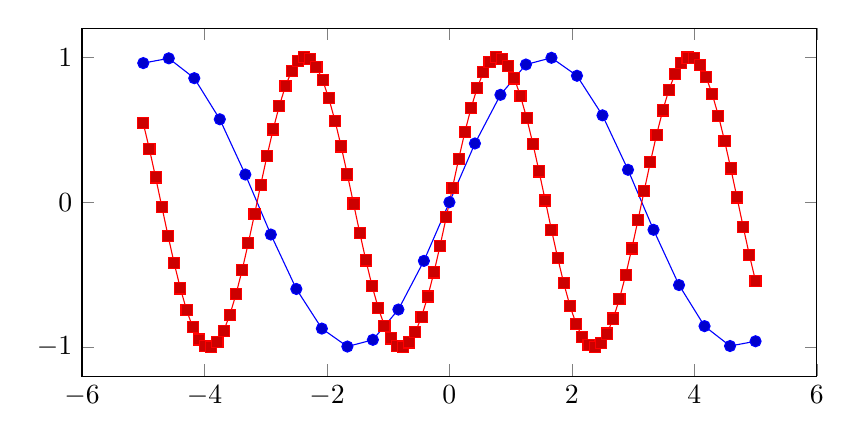
\begin{tikzpicture}
      \begin{axis}[
        width=0.9\textwidth,
        height=6cm,
      ]

        \addplot {sin(deg(x))};
        \addplot+[samples=100] {sin(deg(2*x))};

      \end{axis}
    \end{tikzpicture}
  \end{figure}
\end{frame}


\begin{frame}{3D plots}
\begin{figure}
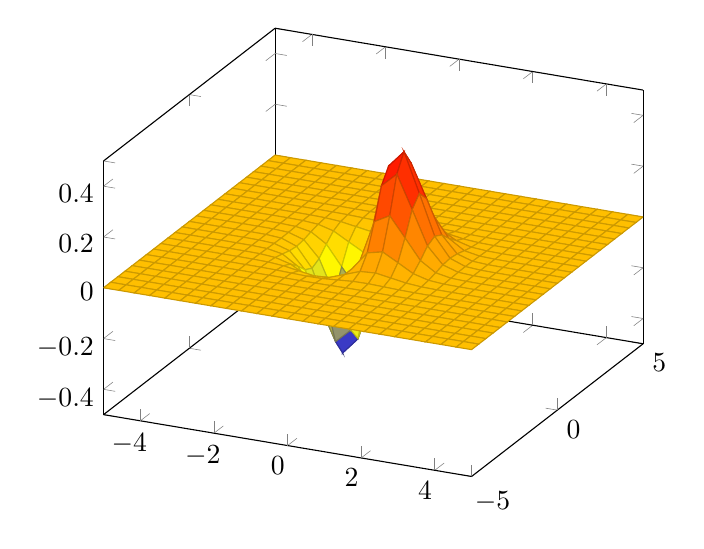
\begin{tikzpicture}
  \begin{axis}
  \addplot3[
      surf,
  ]
  {exp(-x^2-y^2)*x};
  \end{axis}
  \end{tikzpicture}
\end{figure}
\end{frame}
%%%%%%%%%%%%%%%%%%%%%%%%%%%%%%%%%%%%%%%%%%%%%%%%%

\begin{frame}
  \frametitle{tcbb}
  \centering
  \tcbb[0.5]{Fermat's Last Theorem}{
       Fermat's Last Theorem states that
       \[ x^n + y^n = z^n\]
       has no non-zero integer solutions for $x$, $y$ and $z$ when $n > 2$.
  }
\end{frame}

\begin{frame}\frametitle{block}
	\begin{block}{勾X定理:}
		直角三角形的斜边的平方等于两直角边的平方和。
		可以用符号语言表述为:设直角三角形ABC,其中$\angle C=90^\circ $则有
		\begin{equation}
			AB^2=BC^2+AC^2 \int
		\end{equation}
	\end{block}
	\begin{block}{Remark}
		Sample text
	\end{block}
\end{frame}

\begin{frame}
    \frametitle{alertblock}
	\begin{alertblock}{Important theorem}
		Sample text in red box
	\end{alertblock}
\end{frame}

\begin{frame}
    \frametitle{exampleblock}
	\begin{exampleblock} {Exampleblock}
		Sample text in green box. The title of the block is 'Examples'.
	\end{exampleblock}
    \begin{exampleblock} {例1:}
		Sample text in green box. The title of the block is 'Examples'.
	\end{exampleblock}
\end{frame}

\begin{frame}
    \frametitle{examples}
	\begin{examples}
		Sample text in green box. The title of the block is 'Examples'.
	\end{examples}
\end{frame}

\begin{frame}{tcolorbox}  
  \begin{tcolorbox}[title=5.tcolorbox,colframe=red!75!black]
    This is tcolorbox
  \end{tcolorbox}
\end{frame}

\begin{frame}
    \frametitle{5.proof}
    \begin{proof}{}
      This is a proof
    \end{proof}
\end{frame}

\begin{frame}
    \frametitle{自定义tcolorbox1$\to$4}
    \begin{tcolorbox1}[0.8]{tcolorbox1}
      This is tcolorbox1 that I defined
    \end{tcolorbox1}
    \begin{tcolorbox2}[0.86]{tcolorbox2}
      This is tcolorbox2 that I defined
    \end{tcolorbox2}
\end{frame}
\begin{frame}
  \frametitle{}
  \begin{tcolorbox3}[量子力学基本假设1/5]
    \lipsum[4]
  \end{tcolorbox3}
  \end{frame}
  \begin{frame}    
    \begin{tcolorbox4}[量子力学基本假设1/5]
    \lipsum[4]
    \end{tcolorbox4}
\end{frame}

\begin{frame}
    \frametitle{tcbitemize}

    \tcbset{colback=white,arc=0mm,width = (\linewidth-4pt)/4,
    equal height group=AT,before=,after=\hfill,fonttitle=\bfseries}
    
    \noindent
    \foreach \n in {xxx,ggg,AAA,\"Agypten}
    {\begin{tcolorbox}[title=\n,colframe=red!75!black]
      Some content.
    \end{tcolorbox}}
    
    \noindent
    \foreach \n in {xxx,ggg,AAA,\"Agypten}
    {\begin{tcolorbox}[adjusted title=\n,colframe=blue!75!black]
    Some content.
    \end{tcolorbox}}
    
    \begin{tcbitemize}[raster columns=3,raster equal height,
              colframe=red!75!black,colback=red!5!white,fonttitle=\bfseries]
      \tcbitem[squeezed title={Short title}]
      First box
      \tcbitem[squeezed title={This is a very very long title}]
      Second box
      \tcbitem[squeezed title={This title is clearly to long for this application}] Third box
    \end{tcbitemize}
\end{frame}

\begin{frame}{选择题}

  一、单选题(每题2分)\\ \vspace{0.3em}
  1、下列说法正确的是: (\hspace{0.5em} )
  \xxxx{选项 A 的内容}{选项 B 的内容}{选项 C 的内容}{选项 D 的内容} 
  2、下列说法正确的是: (\hspace{0.5em} )
  \xxxx{选项 A 的内容的内容的内容的内容的内容}{选项 B 的内容}{选项 C 的内容}{选项 D 的内容}
\end{frame}

\begin{frame}
  \frametitle{学术讨论}
      %\begin{figure}
         % \centering
         % \subfigure[]{\includegraphics[width=4.5cm]{figs/ds-1.jpeg}}
         % \subfigure[]{\includegraphics[width=4.5cm]{figs/ds-2.jpeg}}
         %\subfigure[]{\includegraphics[width=4.5cm]{figs/ds-3.jpeg}}
          %\caption{} %图片标题
          %\label{fig:1}  
      %    {\color{red} How can electrons be both a particle and a wave?}
      %\end{figure}
\end{frame}

                   %
%                                               %
%%%%%%%%%%%%%%%%%%%%%%%%%%%%%%%%%%%%%%
\begin{frame} [plain]
    \frametitle{}
    \Background[2] 
    \begin{center}
    { {\huge 第八章:统计物理 }}
    \end{center}  
    \addtocounter{framenumber}{-1}   
\end{frame}
%%%%%%%%%%%%%%%%%%%%%%%%%%%%%%%%%%

\begin{frame}
  \frametitle{两个问题决定技术路线}
  \begin{enumerate}
    \item 全同粒子是否不可区分?
  \begin{itemize}
    \item 可区分(定域量子系统) :量子计算+经典统计 $\to $玻尔兹曼统计 
    \item 不可区分(非定域量子系统):量子计算+量子统计
  \end{itemize}
  \begin{figure}[htbp]
    \centering
    \includegraphics[width=0.40\textwidth]{figs/indis.png}
  \end{figure}
    \item 如果不可区分,是费米子还是玻色子?
    \begin{itemize}
      \item 玻色子:量子计算+玻色-爱因斯坦统计
      \item 费米子:量子计算+费米-狄拉克统计
    \end{itemize}
  \end{enumerate} 
\end{frame} 

\section{统计热力学 }

\subsection{微观态与宏观态}

\begin{frame}
  \frametitle{ 1、微观态}
  \alert{单粒子微观态:} 一个能量本征函数描述粒子的一个微观态
  \begin{enumerate}
    \item 量子数法 :记粒子的自由度为 $r$, 则一组$r$个好量子数完全确定一个本征波函数(微观态)比如:氢原子的本征函数由四个量子数构成的组确定
    \[
      \begin{aligned}
        \psi _{nlm_lm_s} &= \left\vert nlm_lm_s \right\rangle \qquad \text{不考虑旋轨耦合} \\ 
        \psi _{nljm} &= \left\vert nljm \right\rangle \qquad \quad \text{考虑旋轨耦合} \\ 
      \end{aligned}\]
    \item 能级法:
     \begin{itemize}
      \item 无简并:一个能级一个本征函数一个微观态
      \item 简并 : 设简并度为$g_l$($l$是能级编号),一个能级包含$g_l$个微观态
     \end{itemize}
  \end{enumerate}
\end{frame} 

\begin{frame}
  \frametitle{}
  \alert{N粒子系统的微观态:} 系统的一个能量本征函数描述一个微观态
  \begin{enumerate}
    \item 占据数分布法 :
    \begin{itemize}
      \item 非定域:一个占据数分布$(a_1 a_2\cdots a_s)$确定一个本征函数一个微观态【$s$是单粒子量子态编号,见第七章例-8】
      \item 定域: "一个占据数分布+一组粒子编号" 确定一个本征函数一个微观态
     \end{itemize}
     \item 相空间法: 
     \begin{itemize}
      \item 定域: 粒子自由度$r$,N系统自由度$f=Nr$, 由于粒子可区分,张开$2f$维相空间($\Gamma$),一个相点确定一个微观态
      \[\varepsilon(q_1,q_2,\cdots q_f; p_1, p_2, \cdots ,p_f)\]
      \item 非定域:粒子自由度$r$,N系统自由度$Nr$,张开$Nr$维相空间,一个相点确定一个微观态
      \[ \left\vert q_1q_2\cdots q_f\right\rangle \]
     \end{itemize}
    \end{enumerate}
\end{frame} 

\begin{frame}
  \frametitle{}
  若依然采用$2f$维相空间,则一个相格确定一个微观态\\
  \begin{figure}[htbp]
    \centering
    \includegraphics[width=0.28\textwidth]{figs/xg.png}
    %\caption{}
      %\label{fig:}
  \end{figure}
  相格体积由不确定性原理给出:
  \[ \Delta q_1 \Delta p_1 \Delta q_2 \Delta p_2 \cdots \Delta q_f \Delta p_f \approx h^f = h^{Nr}\]
\end{frame} 

\begin{frame}
  \frametitle{ 2、宏观态}
  \alert{定义:} 孤立的N粒子系统经过足够长时间弛豫后,必定会自发地到达一种宏观上的平衡状态,此时测量各宏观物理量(比如能量$E$)有确定值,称系统处于一个宏观态。

  ~~\\ 
  \alert{简并度:} 宏观平衡态只是一种热动平衡,实际测量过程是一个宏观短微观长的过程,系统经历了一系列的微观变化。即有大量的微观态参与了这次则量,这些参与态的总数目称为该宏观态的简并度,由于通常以能量来标识宏观态,记为
  \[\Omega(E)\]
  宏观体系能级连续(为区分记为$\varepsilon$), 能量不确定度记为$d \varepsilon$, 简并度记为 
  \[d\Omega(\varepsilon) = \Omega(\varepsilon) d \varepsilon \]
  式中$\Omega(\varepsilon)$,称为态密度。
\end{frame} 

\begin{frame}
  \frametitle{}
  \alert{最概然宏观态:} 简并度取极大值的宏观态,有
  \[\frac{\partial }{\partial E }\Omega(E) =0\]
  ~~\\ 
  \alert{微观态总数目:} 对于确定的宏观态$E$,系统所含微观态总数目为
  \[\Phi(E) = \int_{\varepsilon \le E} \Omega(\varepsilon) d \varepsilon\]
  ~~\\ 
  一个正常的系统,能量是无上限的,宏观态能量越高,则总微观态数目越多,可以证明与能级的简并度($f$)呈幂指数关系(见教材)
  \[\Phi(E) =C E^f\]
\end{frame} 
 
\begin{frame}
  \frametitle{}
  \例[1]{求受限于$V=L^3$系统内的一自由粒子系统在$ε~ε+dε$的能量范围内可实现微观状态数目}
  \解 设粒子质量为$m$, 由于受限,粒子能级是量子化的,量子描述为
  \[ \varepsilon = \frac{\pi ^2 \hbar^2}{2m L^2}(n_x^2 +n_y^2 + n_z^2 )\qquad \implies n_x^2 +n_y^2 + n_z^2 = \left( \frac{L}{\pi \hbar} \sqrt{2m \varepsilon}  \right)^2 \]
  这是一个三维球体,半径为 $ r =  \frac{L}{\pi \hbar} \sqrt{2m \varepsilon} $  \\
  微观态总数目
  \[\Phi(E) = \int_{\varepsilon \le E} \Omega(\varepsilon) d \varepsilon\]
  相当于这个球的体积,考虑到:$n_x, n_y, n_z =1,2,3,\cdots$,只需计算第一象限
  \[\Phi(E) = \frac{1}{8} \cdot\frac{4}{3} \pi r^3 = \frac{\pi}{6} \left( \frac{L}{\pi \hbar} \sqrt{2m \varepsilon}  \right)^3 = \frac{1}{6} \frac{V}{\pi ^2 \hbar^3} (2m)^{3/2} \varepsilon^{3/2} \]
\end{frame} 

 \begin{frame}
   \frametitle{}
  态密度
  \[  \Omega(\varepsilon) =\frac{\mathrm{d}  }{\mathrm{d}\varepsilon}\Phi(E) = \frac{\mathrm{d}  }{\mathrm{d}\varepsilon} \frac{1}{6} \frac{V}{\pi ^2 \hbar^3} (2m)^{3/2} \varepsilon^{3/2} = \frac{3}{2}\cdot\frac{1}{6} \frac{V}{\pi ^2 \hbar^3} (2m)^{3/2} \varepsilon^{1/2} \]
  考虑态密度变化是平滑的,则可实现微观状态数目
  \[\Omega(\varepsilon)  d \varepsilon = \frac{1}{4} \frac{V}{\pi ^2 \hbar^3} (2m)^{3/2} \varepsilon^{1/2} d \varepsilon \]
  若考虑自旋量子数$s$, 则自旋多重度为$2s+1$,即现有每个相格内含$2s+1$个简并的量子态,因此还要乘上这个因子。
 \end{frame} 

 \begin{frame}
   \frametitle{ 3、系综}

   \begin{minipage}[b]{0.49\textwidth}
    \begin{enumerate}
      \item 测得系统能量为$E$,参与测量的微观态数目为$\Omega(E) = \Omega(\varepsilon) d (\varepsilon) $,即相空间的红色区域,区域的每一个相格代表($n_x, n_y, n_z$)代表一个参与测量的微观态。
    \end{enumerate}
    \end{minipage}
    \begin{minipage}[b]{0.49\textwidth}
      \begin{figure}[htbp]
        \centering
        \includegraphics[width=0.92\textwidth]{figs/xz.png}
        %\caption{}
           %\label{fig:}
       \end{figure}
      \end{minipage}
      \begin{enumerate}
        \setcounter{enumi}{1}
        \item 设想红色区域内每一个微观态都是系统的一个思维副本(比如一张像),即一个静态系统,所有的静态系统构成系统的系统,称为系综 
        \item 测量结果是测量时间内的平均值,也是系综内每一个系统参与测量共同贡献的结果,那时间平均等效于系综平均。
      \end{enumerate}
 \end{frame} 

\begin{frame}
  \frametitle{}
为得到一个苹果的准确重量,连续称$\Omega(G)$次,然后取平均值,称为时间平均\\
\begin{figure}[htbp]
  \centering
  \includegraphics[width=0.2\textwidth]{figs/apple.png}
  %\caption{}
    %\label{fig:}
\end{figure}
~~\\ 
复制$\Omega(G)$个苹果构成系综,同时对它们称重并取平均,叫系综平均。\\
\end{frame} 

\begin{frame}
  \frametitle{ 4、宏观量与微观量的关系}
  对宏观系统的某一宏观量进行测量,在这段宏观短微观长的测量时间里,系统经历了大量微观态上的变化。宏观测量值是所有参与测量的微观态对应微观量值的统计平均值。
  \[ \overline{F}_{\text{测}} = \sum _{s=1}^{\Omega(E)} \rho _s F_s = \sum _{s} \rho _s \sum _{i=1}^N f_{si} \]
  \emf[参与态表述:] 式中$s$是参与测量的微观态编号, $F_s$是系统的第$s$个参与态对应力学量$F$的值,$\rho _s$是其参与测量的概率, $f_i$是第$i$个单粒子对应力学量$f$的值

  ~~\\ 
  \emf[系综表述:] $\overline{F}$是系综力学量$F$的平均, $F_s$是系综第$s$个系统力学量$F$的值,$\rho _s$是第$s$个系统的参与概率, $f_i$是系统中第$i$个单粒子对应力学量$f$的值
\end{frame} 

\begin{frame}
  \frametitle{概率的几种表述}
  \begin{itemize}
    \item 参与概率$\rho _s$: 微观态$s$参与测量的概率
    \item 出现概率$\rho _s$: 微观态$s$在测量中出现的概率
    \item 所处概率$\rho _s$: 系统处于微观态$s$的概率
  \end{itemize}
  它们都是等效的。
\end{frame} 

\begin{frame}
  \frametitle{ 5、统计物理根本问题}
  量子力学能计算
  \begin{enumerate}
    \item 单粒子的能级
    \item 粒子在各能级的分布
    \item N粒子系统的态函数(编号$s$),能级(编号$l$)及简并度($g_l$),力学量$F$在$s$态的平均值$F_s$或力学量$F$在$l$能级的平均值$F_l$
  \end{enumerate}
  但是,量子力学不能计算参与概率$\rho _s$ !!!
    
  ~~\\ 
  \emf[统计物理的第一要务:]  \\
  计算量子态参与概率 $\rho _s$,或系统能级的参与概率 $\rho _l$: $$ \rho _l = \sum_{s=1}^{g_l} \rho _s \implies \overline{F}_{\text{测}} = \sum _{l} \rho _l F_l $$
\end{frame} 

\subsection{三大分布}

\begin{frame}
  \frametitle{三种系统}
  为求参与概率$\rho _s$,对物理系统分类:
\begin{enumerate}
  \item 孤立系统:与周围环境无能量交换,无粒子交换, 构成微正则系综  
  \item 封闭系统:与周围环境有能量交换,无粒子交换,构成正则系综 
  \item 开放系统:与周围环境有能量交换,有粒子交换, 构成巨正则系综 
\end{enumerate}
\begin{figure}[htbp]
  \centering
  \includegraphics[width=0.15\textwidth]{figs/xtandhj.png}
  %\caption{}
    %\label{fig:}
\end{figure}
下面针对三种系统,分别求参与概率$\rho _s$($\rho _l$)
\end{frame} 

\begin{frame}
  \frametitle{ 1、孤立系统}
  \alert{等概率原理:}  达到平衡态的微正则系综,各子系统出现的概率相等。或者说当孤立系统达到平衡状态时,各可能的微观状态出现的概率相等。
  \begin{figure}[htbp]
    \centering
    \includegraphics[width=0.2\textwidth]{figs/boltz.png}
    %\caption{}
      %\label{fig:}
  \end{figure}
  玻耳兹曼在1870s年代提出这个基本原理,人们试图想从数学上或物理上进行推导或证明,最后都以失败告终!如今,等概率原理已成为统计物理学最基本的假设。
\end{frame} 


\begin{frame}
  \frametitle{}
  \alert{微正则分布函数:} \\ 
  设处于平衡态的孤立系统的能量为$E$, 则在测量区域$\varepsilon - \varepsilon+ d\varepsilon $内微观态总数为
  $$
  \Omega(E) = \Omega(\varepsilon)  d \varepsilon = \sum_l g_l 
  $$ 
  \alert{参与概率:} \\
  根据等概率原理,它们参与测量的概率是相等的,因此,每一个微观态的参与概率为
  \[ \rho _s = \frac{1}{\Omega(E)} \]
\end{frame} 

\begin{frame}
  \frametitle{ 2、封闭系统}
  封闭系统与周围环境有能量交换,无粒子交换。相当于与一个大热源有接触,因此当达到平衡时,有具有确定(N,V,T)
  \begin{figure}[htbp]
    \centering
    \includegraphics[width=0.16\textwidth]{figs/xzzz.png}
    %\caption{}
      %\label{fig:}
  \end{figure}
  此封闭系统与热源一起构成一个大的孤立系统,设平衡时封闭系统能量为$E$,热源能量为$E_r$,孤立系统能量为$E^0$,有能量关系:
  \[ E + E_r = E^0, \qquad E^0 \gg E\] 
\end{frame} 

\begin{frame}
  \frametitle{}
  当封闭系统与热源相互作用很弱时,有简并度关系:\[ \Omega(E) \cdot \Omega _r(E_r) = \Omega ^0 (E^0), \qquad \Omega ^0 (E^0) \gg \Omega(E)\]
  因为对于封闭系统的一个微观态$s$来说(能量$E_s$),总系统上有$\Omega _r (E_r)$个态与之对应。并且
  \[\Omega _r (E_r) = \Omega _r(E^0 - E_s) \] 
  总系统是孤立系统,一个态的参与概率为
  \[ \rho ^0 _s = \frac{1}{\Omega^0 (E^0)} =c. \]
  $\Omega _r (E_r)$个态的参与概率
  \[ \rho ^0 _s \Omega _r (E_r)  =\rho ^0 _s  \Omega _r (E^0 - E_s)  = \rho _s \qquad \cdots \qquad (1)\]
  这正是封闭系统上微观态$s$的参与概率
\end{frame} 

\begin{frame}
  \frametitle{}
由于 $ E^0 \gg E_s $,可对  $ \ln \Omega _r (E^0 - E_s) $ 做针对$ E_s$的幂级数展开
\[ 
\begin{aligned}
  \ln \Omega _r (E^0 - E_s)  &=  \ln \Omega _r (E^0) + \left(\frac{\partial \Omega _r }{\partial E_r}\right)_{E_r =E^0} (-E_s) +\cdots \\ 
  & \approx \ln \Omega _r (E^0) - \beta  E_s \\
  &= \ln \Omega _r (E^0) - \beta E_s
\end{aligned}  
\] 
两边取e指数,得
\[ \Omega _r (E^0 - E_s) = \Omega _r (E^0) e^{- \beta E_s }\]
代回(1)式,有
\[\rho _s  =\rho ^0 _s  \Omega _r (E^0 - E_s)  =  \frac{\Omega _r (E^0)}{\Omega^0 (E^0)} e^{- \beta E_s}\]
\end{frame} 

\begin{frame}
  \frametitle{}
代入$\Omega(E) \cdot \Omega _r(E_r) = \Omega ^0 (E^0)$, 得态参与概率:
\[\rho _s  =  \frac{1}{\Omega(E)} e^{- \beta E_s}\] 
归一化
\[\sum_s \rho _s  = \frac{1}{\Omega(E)} \sum_s e^{- \beta E_s} =1 \]
得简并度:也称封闭系统的配分函数
\[\Omega(E) = \sum_s e^{- \beta E_s} = Z\]
微观态参与概率:
\[\rho _s  =  \frac{1}{Z} e^{- \beta E_s}\] 
也称$ e^{- \beta E_s}  $为玻尔兹曼因子 
\end{frame} 

\begin{frame}
  \frametitle{}
  \alert{正则分布函数:} \\ 
  设处于平衡态的封闭系统的能量为$E$, 在测量区域$\varepsilon - \varepsilon+ d\varepsilon $内微观态能级为$\{ E_l, \quad (l=1,2,3,\cdots )\}$, 且简并度为$\{ g_l \}$,则配分函数为
  \[ Z= \sum_l g_l e^{- \beta E_l }  = \Omega(E)\]  

  \alert{参与概率:}  \\
  系统能级$ E_l $的参与概率(系统处于能级$ E_l $的概率)为 
  \[ \rho _l  =  \frac{1}{Z} g_l e^{- \beta E_l} \] 
\end{frame} 



\begin{frame}
  \frametitle{ 3、开放系统}
  开放系统与源不仅交换能量还交换粒子,因此粒子数不具确定值
  \begin{figure}[htbp]
    \centering
    \includegraphics[width=0.16\textwidth]{figs/zxjzz.png}
    %\caption{}
      %\label{fig:}
  \end{figure}
  由于源可以很大,粒子数众多,在达到平衡后交换极少量粒子不改变源的温度和化学势,因此体系具有确定的(V,T,$\mu$)。有
  能量关系:
  \[ E + E_r = E^0, \qquad E^0 \gg E\] 
  粒子数关系
  \[ N + N_r = N^0, \qquad N^0 \gg N\]  
\end{frame} 

\begin{frame}
  \frametitle{}
  当系统处于粒子数为N、能量为$E_s$的微观状态$s$ 上时,有简并度关系:
  \[ \Omega(N_s, E_s) \cdot \Omega _r(N_r, E_r) = \Omega ^0, \qquad \Omega ^0 \gg \Omega(N_s, E_s)\]
  因为对于开放系统的一个微观态$s$来说(能量$E_s$),总系统上有$\Omega _r (N_r,E_r)$个态与之对应。并且
  \[\Omega _r (N_r, E_r) = \Omega _r(N^0 - N_s , E^0 - E_s) \] 
  代回,得 
  \[ \Omega(N_s, E_s) \cdot \Omega _r(N^0 - N_s , E^0 - E_s) = \Omega ^0\]
  两端同除1,得
  \[ \rho _{Ns} = \frac{1}{\Omega(N_s, E_s)} = \frac{1}{\Omega ^0}\Omega _r(N^0 - N_s , E^0 - E_s) \qquad \cdots  \quad (2)\]
\end{frame} 

\begin{frame}
  \frametitle{}
由于 $ E^0 \gg E_s, N^0 \gg N_s $,可把  $ \ln \Omega _r(N^0 - N_s , E^0 - E_s)  $ 展开成$N_s, E_s$的幂级数
\[ 
\begin{aligned}
  \ln \Omega _r(N^0 - N_s , E^0 - E_s)  &=  \ln \Omega _r (N^0 , E^0) + \left(\frac{\partial \Omega _r }{\partial E_r}\right)_{E_r =E^0} (-E_s) +\cdots \\ 
  & \qquad + \left(\frac{\partial \Omega _r }{\partial N_r}\right)_{N_r =N^0} (-N_s) +\cdots \\ 
  & \approx \ln \Omega _r (N^0 , E^0) - \alpha  N_s - \beta  E_s 
\end{aligned}  
\] 
两边取e指数,得
\[ \Omega _r(N^0 - N_s , E^0 - E_s) = \Omega _r (N^0 , E^0) e^{- \alpha  N_s - \beta E_s }\]
代回(2)式,有
\[\rho _{Ns}  =  \frac{\Omega _r (N^0 , E^0)}{\Omega^0 } e^{- \alpha  N_s - \beta E_s }\]
\end{frame} 

\begin{frame}
  \frametitle{}
在此
\[\rho  _{Ns}  =  \frac{1}{\Omega(N_s, E_s) } e^{- \alpha  N_s - \beta E_s }\] 
归一化
\[\sum_N^{\infty}\sum_s  \rho  _{Ns} = \frac{1}{\Omega(N_s, E_s) }  \sum_N^{\infty} \sum_s   e^{- \alpha  N_s - \beta E_s } =1 \]
得简并度:也称开放系统的巨配分函数
\[\Omega(N_s, E_s) = \sum_N^{\infty} \sum_s  e^{- \alpha  N_s - \beta E_s } = \Xi \]
微观态参与概率:
\[\rho  _{Ns}  =  \frac{1}{\Xi} e^{- \alpha  N_s - \beta E_s }\] 
也称$ e^{- \alpha  N_s - \beta E_s }$为吉布斯因子 
\end{frame} 

\begin{frame}
  \frametitle{}
  \alert{巨正则分布函数:} \\ 
  设处于平衡态的开放系统粒子数为$N$能量为$E$, 在测量区域$\varepsilon - \varepsilon+ d\varepsilon $内微观态能级为$\{ E_l, \quad (l=1,2,3,\cdots )\}$, 粒子数为$\{ N_l \}$ 且简并度为$\{ g_l \}$,则巨配分函数为
  \[ \Xi= \sum_l g_l e^{- \alpha  N_l - \beta E_l }  = \Omega(N, E)\]  

  \alert{参与概率:}  \\
  系统处于粒子数为$ N_l$,能量为$ E_l $的第$l$能级的概率为 
  \[ \rho _l  =  \frac{1}{\Xi} g_l e^{- \alpha  N_l - \beta E_l } \] 
\end{frame} 

\begin{frame}
  \frametitle{}
\例[2]{由N个全同粒子构成的封闭系统,设单粒子可能的状态有两个,能量分别为0,$\varepsilon$, 求体系的能量平均值。}
\解 (1)系统能级法
\begin{itemize}
  \item 系统能级$E_l$:$~0~,~\varepsilon~, ~2\varepsilon~, ~\cdots~ , ~l\varepsilon~, ~\cdots~, ~N \varepsilon~ $ 
  \item 简并度$\quad~ g_l$:$~1,~C_N^1, ~C_N^2, \cdots , ~C_N^l, ~\cdots, ~C_N^N $
\end{itemize}
封闭系统的配分函数
\[\begin{aligned}
 Z = \sum_l g_l e^{-\beta E_l} = \sum_l C_N^l e^{-\beta \varepsilon l} = (1+e^{-\beta \varepsilon})^N \\ 
\end{aligned} 
  \]
  能级参与概率
  \[ \rho _l = \frac{1}{Z} g_l e^{-\beta E_l} \]
  能量平均值
  \[ \overline{E} = \sum_{l=0}^N \rho _l E_l = \sum_{l=0}^N\frac{1}{(1+e^{-\beta \varepsilon})^N } C_N^l l\varepsilon  e^{-\beta l\varepsilon} \]
\end{frame} 

\begin{frame}
  \frametitle{}
  (2)单粒子能级法
  \begin{itemize}
    \item 单粒子能级$\varepsilon_l$:$~0~,~\varepsilon~$ 
    \item 简并度$\quad\quad~ g_l$:$~1,~1$
  \end{itemize}
  单粒子配分函数 
  \[z_1 = \sum_l g_l e^{-\beta \varepsilon_l} = 1+ e^{-\beta \varepsilon} \]
  系统配分函数
  \[Z = (z_1)^N =  (1+e^{-\beta \varepsilon})^N\]
\end{frame} 

\subsection{热力学统计诠释}

\begin{frame}
  \frametitle{ 1、热力学第一定律}
  表述:系统内能的增加等于系统吸收的热量和对系统所作的功的总和 
\[ dU = dQ - dW = dQ- Y dX \quad \cdots \quad (1) \]
令系统是达到平衡状态的封闭系统,它处于能级$E_l$的概率为$\rho _l$,能量平均值为
\[ U = \overline{E} = \sum_l \rho _l E_l\]
求微分
\[ dU = \sum_l E_l d\rho _l + \sum_l \rho _l d E_l \quad \cdots \quad (2)\]
\end{frame} 

\begin{frame}
  \frametitle{}
比较(1)(2)式,并令  
\[ dQ = \sum_l E_l d\rho _l, \qquad  -dW = \sum_l \rho _l d E_l \]
统计意义:
\begin{itemize}
  \item 系统吸收热量,系统处于高更能级的概率增加,能量平均值增加。
  \item 对系统作功,系统能谱被提升,能量平均值增加。
\end{itemize}
\[
\begin{aligned}
  -Y dX &= \sum_l \rho _l d E_l  \\
  Y &= - \sum_l \rho _l \frac{\partial E_l }{\partial X}    \\ 
\end{aligned}\]
\begin{itemize}
  \item 广义力是各能级对广义坐标微商的统计平均
\end{itemize}
\end{frame} 

\begin{frame}
  \frametitle{ 2、温度和熵 }
  温度和熵与两系统的平衡有关。我们把一个达到平衡状态的孤立系统分成两个子系统$A_1, A_2$, 它们之间可交换能量不交换粒子
  \begin{figure}[htbp]
    \centering
    \includegraphics[width=0.4\textwidth]{figs/tands.png}
    %\caption{}
      %\label{fig:}
  \end{figure}
  约束条件
  \[ E_1 + E_2 = E^0 =c.\]
\end{frame} 

\begin{frame}
  \frametitle{}
  孤立系统的微观状态数
  \[ \Omega^0 = \Omega _1 (E_1)\Omega _2 (E_2) = \Omega _1 (E_1)\Omega _2 (E^0 - E_1) \]
  平衡态是最概然宏观态
  \[ 
  \begin{aligned}
   \frac{\partial \Omega^0 }{\partial E_1 } =0 &= \Omega _2 (E_2) \frac{\partial \Omega _1 (E_1) }{\partial E_1 }  + \Omega _1 (E_1)\frac{\partial }{\partial E_1 }\Omega _2 (E^0 - E_1) \\
   &= \Omega _2 (E_2) \frac{\partial \Omega _1 (E_1) }{\partial E_1 }  - \Omega _1 (E_1)\frac{\partial }{\partial E_1 }\Omega _2 (E^0 - E_1) \\
   &= \Omega _2 (E_2) \frac{\partial \Omega _1 (E_1) }{\partial E_1 }  - \Omega _1 (E_1) \frac{\partial E_1 }{\partial E_2 } \frac{\partial }{\partial E_1 }\Omega _2 (E_2)  \\
   &=  \Omega _2 (E_2) \frac{\partial \Omega _1 (E_1) }{\partial E_1 }  - \Omega _1 (E_1) \frac{\partial }{\partial E_2 }\Omega _2 (E_2)  \\
  \text{得:} \quad \Omega _2 (E_2) \frac{\partial \Omega _1 (E_1) }{\partial E_1 }  &= \Omega _1 (E_1) \frac{\partial }{\partial E_2 }\Omega _2 (E_2) 
  \end{aligned}\]
\end{frame} 

\begin{frame}
  \frametitle{}
整理
$$
 \frac{1}{\Omega _1 (E_1) }\frac{\partial \Omega _1 (E_1) }{\partial E_1 }  = \frac{1}{\Omega _2 (E_2)} \frac{\partial }{\partial E_2 }\Omega _2 (E_2) 
$$ 
得
$$
\begin{aligned}
\frac{\partial \ln \Omega _1 (E_1) }{\partial E_1 }  &= \frac{\partial \ln \Omega _2 (E_2)}{\partial E_2 } 
\\ 
\left(\frac{\partial \ln \Omega _1 (N_1,E_1,V_1) }{\partial E_1 }\right)_{N_1,V_1}  &= \left(\frac{\partial \ln \Omega _2 (N_2,E_2,V_2)}{\partial E_2 } \right)_{N_2,V_2}  
\end{aligned}$$ 
得平衡条件 
\[ \beta _1 = \beta _2\]
\end{frame} 

\begin{frame}
  \frametitle{}
  等式现端同乘$k_B$
  $$
  \begin{aligned}
  \left(\frac{\partial k_B \ln \Omega _1 (N_1,E_1,V_1) }{\partial E_1 }\right)_{N_1,V_1}  &= \left(\frac{\partial k_B \ln \Omega _2 (N_2,E_2,V_2)}{\partial E_2 } \right)_{N_2,V_2}  \\
  \left(\frac{\partial S_1 }{\partial E_1 }\right)_{N_1,V_1}  &= \left(\frac{\partial S_2}{\partial E_2 } \right)_{N_2,V_2}  \\
  \end{aligned}$$ 
  得平衡条件
  \[\frac{1}{T_1} = \frac{1}{T_2}\]
  因此,有
 
\end{frame} 

\begin{frame}
  \frametitle{}
  \[ \boxed{\beta = \frac{1}{ k_B T} = \left(\frac{\partial \ln \Omega (N,E,V) }{\partial E_1 }\right)_{N,V}, \quad S = k_B \ln \Omega }\]
  左端是热力学量,右端是统计量 

  ~~\\ 
  统计意义:
  \begin{itemize}
    \item $\beta $: N,V不变时,系统微观态数目随能量变化时的相对变化量。相对变化量越大,则温度越低
    \item $S$: 熵是状态量,是系统微观状态数的量度。微观状态数越多,则熵越大。 
  \end{itemize}
\end{frame} 

\begin{frame}
  \frametitle{ 3、热力学第二定律}
 \emf[熵增加原理:] 在任何自然过程中,一个孤立系统的熵永不自动减少,熵在可逆过程中不变,在不可逆过程中增加。

 ~~\\ 
 统计意义:
  \begin{itemize}
    \item 熵增加: 微观状态数增加
    \item 熵增加原理: 在任何自然过程中,宏观孤立系统总是自发地从微观状态数少的态向微观状态数多的态演化
    \item 宏观过程不可逆: 微观演化是可逆的幺正变换过程,宏观演化是向着最概然宏观态的不可逆过程,宏观不可逆是概率导致的不可逆。
  \end{itemize}
\end{frame} 

\begin{frame}
  \frametitle{ 4、热力学第三定律}
  \emf[表述:]绝对零度不可达到但可以无限趋近,或与任何等温可逆过程相联系的熵变,随着温度的趋近于绝对零度而趋近于零,或当一个系统的温度趋于绝对零度时,其熵趋于定值或保持不变。

 ~~\\ 
 统计意义:
  \begin{itemize}
    \item 温度趋近于绝对零度: 系统趋于基态
    \item 基态:系统的微观状态数目为“1”
    \item 熵变趋零:
\[ S = k_B \ln \Omega, \qquad S_{T \to 0} = k_B \ln (\Omega \to 1) = 0 \]
  \end{itemize}
\end{frame} 

\subsection{热力学量的统计计算}

\begin{frame}
  \frametitle{ 1、内能}
  以正则系综为例,先计算配分函数Z
  \[ Z = \sum_s e^{-\beta E_s}\]
  \[ \frac{\partial Z}{\partial \beta } = \frac{\partial }{\partial \beta } (\sum_s e^{-\beta E_s})
    = \sum_s \frac{\partial }{\partial \beta } ( e^{-\beta E_s}) =  - \sum_s \frac{\partial }{\partial \beta } E_s e^{-\beta E_s} \]
  热力学内能,就是能量的平均值,
  \[ U \equiv \overline{E} \equiv  \sum_s \rho _s E_s \]
  代入态参与概率
  \[ \begin{aligned}
    U = \sum_s \frac{1}{Z} e^{-\beta E_s} E_s = -\frac{1}{Z} ( - \sum_s E_s e^{-\beta E_s} )  = - \frac{1}{Z} \frac{\partial Z}{\partial \beta } \\ 
  \end{aligned}\]
\end{frame} 

\begin{frame}
  \frametitle{}
  得内能计算公式
  \[ \boxed{U = -  \frac{\partial \ln Z}{\partial \beta }} \]
  只要求得系统的配分函数$Z$,就能获得系统的内能。
\end{frame} 

\begin{frame}
  \frametitle{ 2、 广义力 }
  以正则系综为例,先计算配分函数Z
  \[ Z = \sum_s e^{-\beta E_s}\]
  \[ \frac{\partial Z}{\partial X } = \frac{\partial }{\partial E_s} (\sum_s e^{-\beta E_s}) \frac{\partial E_s}{\partial X } 
    = - \beta \sum_s \frac{\partial E_s}{\partial X } e^{-\beta E_s} \]
  由前可行,广义力是各能量对广义坐标微商的统计平均 
  \[Y \equiv  \overline{(\frac{\partial E_s}{\partial X })} \equiv  - \sum_l \rho _l \frac{\partial E_l }{\partial X} \equiv - \sum_s \rho _s \frac{\partial E_s }{\partial X} = - \frac{1}{Z} \sum_s \frac{\partial E_s }{\partial X} e^{-\beta E_s}  = \frac{1}{\beta} \frac{1}{Z} \frac{\partial Z}{\partial X }\] 
\end{frame}

 \begin{frame}
   \frametitle{}
解得广义力计算公式
\[ \boxed{Y = \frac{1}{\beta} \frac{\partial \ln Z}{\partial X }} \]
只要求得系统的配分函数$Z$,就能获得系统的广义力。具体如:
\[ \boxed{p = \frac{1}{\beta} \frac{\partial \ln Z}{\partial V }}, \quad  \boxed{\mu = \frac{1}{\beta} \frac{\partial \ln Z}{\partial N }} \]
 \end{frame} 

\begin{frame}
  \frametitle{ 3、熵 }
  以正则系综为例,先计算配分函数Z
  \[\Omega (N,V,T) = Z = \sum_s e^{-\beta E_s} =Z(\beta, E_s ) = Z(\beta, X )\]
  \[ d \ln Z  = \frac{\partial \ln Z }{\partial X } dX + \frac{\partial \ln Z }{\partial \beta } d \beta  \]
  代入 $ Y = \frac{1}{\beta} \frac{\partial \ln Z}{\partial X }, \qquad U = -  \frac{\partial \ln Z}{\partial \beta } $, 得
  \[ d \ln Z  = \beta Y dX -U d \beta  \]
  考虑到热力学公式 $ dU = TdS - YdX $, 得 
  \[ d \ln Z  = \beta (Y dX + dU) - d(\beta U )- U d \beta  \]
\end{frame} 

\begin{frame}
  \frametitle{}
整理,得
\[ d \ln Z  = \beta TdS - d (\beta U) \]
代入 $\beta T = \frac{1}{k_B}$, 得
\[ d \ln Z  = \frac{1}{k_B} dS - d (\beta U) \]
整理,得
\[ dS = k_B \left[ d \ln Z + d (\beta U) \right] \]
解得 
\[ S = k_B \left[  \ln Z +  \beta U \right] \]
代入 $U = -  \frac{\partial \ln Z}{\partial \beta } $, 得 
\[ \boxed{S = k_B \left[  \ln Z -  \beta \frac{\partial \ln Z}{\partial \beta }  \right]} \]
\end{frame} 

\begin{frame}
  \frametitle{ 4、自由能}
  有热力学公式
  \[ F \equiv  U - TS \]
  代入$S = k_B \left[  \ln Z +  \beta U \right]$, 得 
  \[ F =  U - k_BT \left[  \ln Z +  \beta U \right] \]
  代入$\beta = \frac{1}{k_B T} $, 得 
  \[ \boxed{F =  - k_BT \ln Z }\]
  ${\color{red}\star}$ 一切热力学量都可由配分函数Z求得!配分函数正是可参与微观态总数目
\end{frame} 

\begin{frame}
  \frametitle{}
当然,开放系统的一切热力学量都可由巨配分函数$\Xi$求得!(推导略) 
\[
\begin{aligned}
  \overline{N} &= - \frac{\partial }{\partial \alpha } \ln \Xi \\
U &= - \frac{\partial }{\partial \beta} \ln \Xi \\
Y &= \frac{1}{\beta} \frac{\partial }{\partial X} \ln \Xi \\
S &= k_B [ \ln \Xi + \beta U + \alpha \overline{N} ]\\
\end{aligned} 
  \]
  ${\color{red}\star}$ 求解(巨)配分函数是统计物理学最基本的技能!
\end{frame} 

\begin{frame}
  \frametitle{}
  \例[3]{对于近独立全同玻色子开放系统,求任意单粒子态上粒子的平均占据数}
  \解 设任意单粒子态被一个粒子占据时,贡献系统能量$\varepsilon$, 否则贡献零。
\begin{table}[htbp]
  \centering\begin{tabular}{ccccccc}
    占据数($N$): & ~0~ & ~1~ & ~2~ & $~\cdots~$ & ~n~ & $\cdots$ \\
    能量 ($E_s$): &  0 & $\varepsilon$ & 2 $\varepsilon$ & $\cdots$ & n$\varepsilon$ & $\cdots$ \\
  \end{tabular}
\end{table}
巨配分函数:$$ 
\begin{aligned}
  \Xi = \sum_{N} ^\infty \sum_{E_s} e^{-\alpha N -\beta E_s}  
  = \sum_{n=0}^\infty e^{-\alpha n -\beta n \varepsilon }  
  = \sum_{n=0}^\infty e^{-n(\alpha +\beta \varepsilon)} 
  = \sum_{n=0}^\infty \left(e^{-(\alpha +\beta \varepsilon)}\right)^n 
\end{aligned}
$$ 
由展开式
\[ \frac{1}{1-x} = \sum_{n=0}^{\infty} x^n\]
\end{frame} 

\begin{frame}
  \frametitle{}
得
\[ \Xi = \frac{1}{1-e^{-(\alpha +\beta \varepsilon)}}\]
代入平均数公式
\[
\begin{aligned}
\overline{N} &= - \frac{\partial }{\partial \alpha } \ln \Xi \\
&= - \frac{\partial }{\partial \alpha } \ln (\frac{1}{1-e^{-(\alpha +\beta \varepsilon)}}) \\
&= - (1-e^{-(\alpha +\beta \varepsilon)})\frac{\partial }{\partial \alpha }  (\frac{1}{1-e^{-(\alpha +\beta \varepsilon)}}) \\
&= (1-e^{-(\alpha +\beta \varepsilon)}) \frac{1}{[1-e^{-(\alpha +\beta \varepsilon)}]^2} e^{-(\alpha +\beta \varepsilon)}
\end{aligned} 
  \]
\end{frame} 

\begin{frame}
  \frametitle{}
  \[
    \begin{aligned}
    \overline{N} 
    &=\frac{1}{1-e^{-(\alpha +\beta \varepsilon)}} \cdot \frac{1}{e^{(\alpha +\beta \varepsilon)}}\\
    &= \frac{1}{e^{(\alpha +\beta \varepsilon)}-1}
    \end{aligned} 
      \]
  得,玻色子在能量为$\varepsilon$的单粒子态上的平均占据数
\[ \boxed{f_{B.E} =  \frac{1}{e^{(\alpha +\beta \varepsilon)}-1}}\]
随着能量的变化,构成能谱上的占据数分布, 称为玻色-爱因斯坦分布
\end{frame} 

\begin{frame}
  \frametitle{}
  \例[4]{对于近独立全同费米子开放系统,求任意单粒子态上粒子的平均占据数}
  \解 设如果这个单态被一个粒子占据时贡献系统能量的能$\varepsilon$, 否则贡献零。考虑到泡利不相容原理, 有
\begin{table}[htbp]
  \centering\begin{tabular}{ccccccc}
    占据数($N$): & ~0~ & ~1~ \\
    能量 ($E_s$): &  0 & $\varepsilon$\\
    吉普斯因子: & 1 & $e^{-\alpha -\beta \varepsilon }$ 
  \end{tabular}
\end{table}
巨配分函数:$$ 
\begin{aligned}
  \Xi = \sum_{N} ^n \sum_{E_s} e^{-\alpha N -\beta E_s}  
  &= 1+ e^{-\alpha -\beta \varepsilon }
\end{aligned}
$$ 
\end{frame} 

\begin{frame}
  \frametitle{}
代入平均数公式
\[
\begin{aligned}
\overline{N} &= - \frac{\partial }{\partial \alpha } \ln \Xi \\
&= - \frac{\partial }{\partial \alpha } \ln (1+ e^{-\alpha -\beta \varepsilon }) \\
&= - \frac{1}{1+ e^{-\alpha -\beta \varepsilon }}\frac{\partial }{\partial \alpha } (1+ e^{-\alpha -\beta \varepsilon }) \\
&= \frac{1}{1+ e^{-\alpha -\beta \varepsilon }}e^{-\alpha -\beta \varepsilon } \\
&= \frac{1}{e^{(\alpha +\beta \varepsilon)}+1}
\end{aligned} 
  \]
得,费米子在能量为$\varepsilon$的单粒子态上的平均占据数。
\[ \boxed{f_{F.D} =  \frac{1}{e^{(\alpha +\beta \varepsilon)}+1}}\]
随着能量的变化,构成能谱上的占据数分布, 称为费米-狄拉克分布
\end{frame} 

\section{玻尔兹曼统计 }

\subsection{玻尔兹曼分布}
\begin{frame}
  \frametitle{ 1、玻尔兹曼分布函数}
  玻色子分布在单粒子态上的粒子数 ($0 \le f_{B.E} < +\infty $)
  \[f_{B.E} =  \frac{1}{e^{(\alpha +\beta \varepsilon)}{\color{red} -1}}\]
  费米子分布在单粒子态上的粒子数 ($0 \le f_{B.E} \le 1 $)
  \[f_{F.D} =  \frac{1}{e^{(\alpha +\beta \varepsilon)}{\color{red} +1}}\]
  区别的根源在于不相容原理。不相容原理又源于量子全同粒子不可区分。
\end{frame} 

\begin{frame}
  \frametitle{}
  \begin{minipage}[b]{0.49\textwidth}
   对于定域量子系统来说,不可区分性消失, 则玻色分布和费米分布应相同, 即当 $e^\alpha \gg  1$时, 有
  \[\frac{1}{e^{(\alpha +\beta \varepsilon)}{\color{red} \pm 1}} = \frac{1}{e^{(\alpha +\beta \varepsilon)}}\]
  回归经典分布, 即玻尔兹曼分布:($0 \le f_{B.E} \ll  1 $)
  \[\boxed{f_{B} = e^{-(\alpha +\beta \varepsilon)}}\]
  \end{minipage}
\begin{minipage}[b]{0.49\textwidth}
\begin{figure}[htbp]
  \centering
  \includegraphics[width=0.95\textwidth]{figs/threedis.png}
  %\caption{}
    %\label{fig:}
\end{figure}
\end{minipage}
定域量子系统中, 所有粒子的波函数都没有交叠,是粒子数密度是极小的。是非简并稀薄气体。 
\end{frame} 

\begin{frame}
  \frametitle{}
  \emf[几个重要的计算公式:] 

  ~~\\ 
  在$\varepsilon - \varepsilon + d \varepsilon $区域, 微观态的总数目
  \[ \Omega(E) = d\Omega(\varepsilon) = \Omega(\varepsilon) d \varepsilon \]
  在$\varepsilon - \varepsilon + d \varepsilon $区域, 总占据粒子数
  \[ d N(\varepsilon) = f_{B} d\Omega(\varepsilon) = f_{B} \Omega(\varepsilon) d \varepsilon \]
  系统的总粒子数
  \[ N = \int d N(\varepsilon) = \int_{\varepsilon} f_{B} \Omega(\varepsilon) d \varepsilon\]
  系统的能量
  \[ U= \overline{E} = \int \varepsilon d N(\varepsilon) = \int_{\varepsilon} f_{B} \Omega(\varepsilon) \varepsilon d \varepsilon\]
\end{frame} 

\begin{frame}
  \frametitle{ 2、非简并条件}
  定域量子系统的总粒子数:
  \[ \begin{aligned}
    N &= \int_{\varepsilon} f_{B} d\Omega(\varepsilon) \\ 
    &= \int_{\varepsilon} e^{-(\alpha +\beta \varepsilon)} \frac{1}{4} \frac{V}{\pi ^2 \hbar^3} (2m)^{3/2} \varepsilon^{1/2} d \varepsilon \\
    &= V \left( \frac{2 \pi m k_B T}{h^2} \right)^{3/2} e^{-\alpha}
  \end{aligned}\]
  得非简并条件:
  \[ e^{\alpha} = \frac{V}{N} \left( \frac{2 \pi m k_B T}{h^2} \right)^{3/2} = 
  \frac{1}{n} \left( \frac{2 \pi m k_B T}{h^2} \right)^{3/2}  \gg 1\]
  即要求:(1)粒子数密度$n$很小, (2)粒子质量$m$很大, (3)温度$T$很高。
\end{frame} 

\begin{frame}
  \frametitle{}
一个自由度上的能量
\[  \frac{\overline{E}}{f} = k_B T \]
粒子的自由度为三, 因此粒子的能量
\[ \varepsilon = 3 k_B T \approx \pi k_B T\]
粒子的热波长
\[ \lambda = \frac{h}{p} = \frac{h}{\sqrt{2m\varepsilon } } = \frac{h}{2 \pi m k_B T} \]
代回,有
\[ e^{\alpha} = \frac{1}{n} \frac{1}{\lambda ^3} \gg 1 \qquad \implies \qquad \lambda \ll \frac{1}{n^{1/3}}\]
即:粒子的热波长(德布罗意波长)要远远大于粒子的平均自由程, 因此粒子的波动性可以忽略不计!
\end{frame} 

\begin{frame}
  \frametitle{ 3、配分函数}
  定域量子系统的总粒子数:
  \[ \begin{aligned}
    N = \int_{\varepsilon} f_{B} \Omega(\varepsilon) d \varepsilon  
    = \int_{\varepsilon} e^{-\alpha -\beta \varepsilon} \Omega(\varepsilon) d \varepsilon 
    = e^{-\alpha} \int_{\varepsilon} e^{-\beta \varepsilon} \Omega(\varepsilon) d \varepsilon 
  \end{aligned}\]
  考虑到 $\varepsilon$ 是单粒子能级,应该分立
  \[ \int_{\varepsilon} e^{-\beta \varepsilon} \Omega(\varepsilon) d \varepsilon 
  = \int_{\varepsilon} g_l e^{-\beta \varepsilon _l }  d \varepsilon_l 
  = \sum_l  g_l e^{-\beta \varepsilon _l } = z_1
  \]
  正是单粒子系统的正则配分函数 $z_1$! 对应的单粒子系统正则分布为
  \[ \rho _1 = \frac{1}{z_1} e ^ {-\beta \epsilon} \]
\end{frame} 

\begin{frame}
  \frametitle{}
量子正则系统的配分函数为(定域非定域都一样)
\[ Z = (z_1)^N \]
经典正则系统的配分函数为:
\[ \boxed{Z = \frac{1}{N!} (z_1)^N}  \]
并称$ \frac{1}{N!}  $为吉布斯校正因子。源于全同性简并! 
\end{frame} 

\begin{frame}
  \frametitle{}
  把$z_1$ 代入总粒子数计算式
  \[ N = e^{-\alpha} \int_{\varepsilon} e^{-\beta \varepsilon} \Omega(\varepsilon) d \varepsilon  = e^{-\alpha} z_1 \]
  得\[ e^{-\alpha} = \frac{N}{z_1}\]
  代入玻尔兹曼分布公式
  \[ f_B = e^{-\alpha -\beta \varepsilon} = \frac{N}{z_1} e^{ -\beta \varepsilon} = N \rho _1 \]
  单粒子占据单能态$\varepsilon$的概率乘上总粒子数,正是单能态上粒子的平均占据数。
\end{frame} 

\subsection{应用举例}

\begin{frame}
  \frametitle{}
  \例[5]{试用玻尔兹曼分布导出理想气体物态方程
  \[ PV = Nk_B T\]}
  \解 理想气体可采用定域近独立全同粒子模型, 单粒子能量
  \[ \varepsilon = \frac{p^2}{2m } = \frac{1}{2m} (p_x^2 +p_y^2 + p_z^2)\]
代入单粒子配分函数公式
$$ z_1 =\int e^{-\beta \varepsilon} d \Omega  = \int e^{- \frac{\beta}{2m} (p_x^2 +p_y^2 + p_z^2)} \frac{dxdydzdp_xdp_y dp_z}{h^3} $$ 
\end{frame} 

\begin{frame}
  \frametitle{}
空间积分,得
\[ 
  \begin{aligned}
    z_1 &=\frac{V}{h^3}\int e^{- \frac{\beta}{2m} (p_x^2 +p_y^2 + p_z^2)} dp_xdp_y dp_z  \\ 
&= \frac{V}{h^3}\int e^{- \frac{p_x^2}{2mk_BT}}dp_x \int e^{- \frac{p_y^2}{2mk_BT}}dp_y \int e^{- \frac{p_z^2}{2mk_BT}}dp_z  \\
&= \frac{V}{h^3}\left(\int_{-\infty}^\infty e^{- \frac{p_x^2}{2mk_BT}}dp_x\right)^3 \\
&= \frac{V}{h^3} (2\pi mk_BT)^{3/2}  \qquad \leftarrow \int_{-\infty}^\infty e^{-x^2 dx} = \sqrt{\pi} \\
&= e^\alpha N
  \end{aligned}
\]
${\color{red}\star}$ 以后可直接写出, 这是必然的!
\end{frame} 

\begin{frame}
  \frametitle{}
系统的配分函数为
\[ Z = \frac{1}{N!} (z_1)^N = \frac{V^N}{N!} (k_BT)^{3N/2} \left(\frac{2\pi m}{h^2}\right)^{3N/2}  \]
因此
\[ \ln Z = N \ln V +\frac{3}{2}N \ln (k_BT) + \frac{3}{2} N \ln\left(\frac{2\pi m}{h^2}\right) - \ln N!  \]
代入压强公式
\[ P= \frac{1}{\beta} \frac{\partial \ln Z}{\partial V} = \frac{1}{\beta} N \frac{1}{V} = \frac{Nk_B T }{V}\]
得
\[ PV = Nk_B T\]
\textcolor{red}{结束!}
\end{frame} 

\begin{frame}
  \frametitle{}
  \例[6]{试基于玻尔兹曼分布函数导出麦克斯韦速度分布函数}
  \解 
  由总粒子数公式
\[ 
  \begin{aligned}
    N &= \int f_{B} d\Omega(\varepsilon) \\ 
   &= \int e^{-\alpha -\beta \varepsilon } d\Omega(\varepsilon) \\
   &= \int e^{-\alpha }e^{-\beta \frac{1}{2}m (v_x^2 + v_y^2 + v_z^2 )} \frac{1}{h^3} dxdydzdp_xdp_y dp_z \\
   &= \int e^{-\alpha } e^{-\beta \frac{1}{2}m (v_x^2 + v_y^2 + v_z^2 )} \frac{m^3}{h^3} dxdydzdv_xdv_y dv_z \\
   &= A \int e^{-\frac{m}{2k_B T}v_x^2} d v_x \int e^{-\frac{m}{2k_B T}v_y^2} d v_y \int e^{-\frac{m}{2k_B T}v_z^2} dv_z   
  \end{aligned}  \]
  得麦克斯韦速度分布函数
  \[ f(v_i) = A' e^{-\frac{m}{2k_B T}v_i^2}, \quad  i = x,y,z  \]
\end{frame} 

\begin{frame}
  \frametitle{}
  \例[7]{试基于玻尔兹曼分布函数导出麦克斯韦速率分布函数}
  \解 
  由总粒子数公式,得
  \[ 
  \begin{aligned}
    N &= \int f_{B} d\Omega(\varepsilon) \\ 
   &= \int e^{-\alpha -\beta \varepsilon } d\Omega(\varepsilon) \\
   &= \int e^{-\alpha }e^{-\beta \frac{1}{2}mv^2} v^2 \sin \theta d v d \theta d\varphi \\
   &= B\int e^{-\beta \frac{1}{2}mv^2} v^2 d v \\
   &= B\int e^{- \frac{mv^2}{k_BT}} v^2 d v 
  \end{aligned}  \]
  得麦克斯韦速率分布函数
  \[  f(v) = B e^{- \frac{mv^2}{k_BT}} v^2  \]
\end{frame} 

\begin{frame}
  \frametitle{}
平均速率
\[ \overline{v} = \int v f(v) dv = \int B e^{- \frac{mv^2}{k_BT}} v^3 dv\]
最概然速率
\[ \frac{\mathrm{d}f(v)}{\mathrm{d} v}= 0 \implies v_{m} \]
方均根速率
\[ \overline{v^2} = \int v^2 f(v) dv = \int B e^{- \frac{mv^2}{k_BT}} v^4 dv\]
\[ \implies v_s = \sqrt{\overline{v^2}} \] 
比率:
\[ \boxed{v_s: \overline{v} : v_{m} = \sqrt{\frac{3}{2}} : \frac{2}{\sqrt{\pi}} : 1}  \]
\end{frame} 

\begin{frame}
  \frametitle{}
  \例[8]{试基于能量均分定理求单原子分子理想气体的热容量}
  \解 由能量均分定理:理想气体在达到热平衡后,每个运动模式(平移,旋转)的分子动能都是 $\frac{1}{2}k_BT$,
  单原子分子哈密顿所含平方项:平动 3 个。粒子的平均能量为
  \[ \overline{\varepsilon }  = \frac{3}{2}k_BT\]
  设系统含N个粒子, 则系统的内能为
  \[ U= \frac{3}{2} N k_BT\]
  热容量指物体温度每升高1度所吸收的热量,也称比热 \\
  定容比热: 
  \[ C_V = \left(\frac{\partial U}{\partial T }\right)_V = \frac{3}{2} N k_B\]
\end{frame} 

\begin{frame}
  \frametitle{}
  定压比热:
  \[ C_P = C_V + N k_B = \frac{5}{2} N k_B\] 
  比值: 
  \[\gamma = \frac{C_P}{C_V} = \frac{5}{3} = 1.667 \]
  实验事实: 氦气在 291K时的比值为1.660
\end{frame} 

\begin{frame}
  \frametitle{}
  \例[9]{试基于能量均分定理求双原子分子理想气体的热容量}
  \解 双原子分子哈密顿所含平方项: 平动 3 个, 转动 2个, 一维简谐振动 2个\\
  粒子的平均能量为
  \[ \overline{\varepsilon }  = \frac{7}{2}k_BT\]
  设系统含N个粒子, 则系统的内能为
  \[ U= \frac{7}{2} N k_BT\]
  比热: 
  \[ C_V = \frac{7}{2} N k_B, \qquad C_P = \frac{9}{2} N k_B\]  
  比值: 
  \[\gamma = \frac{C_P}{C_V} = \frac{9}{7} = 1.29 \]
  实验事实: 氢气体在 289K 时的比值为1.407
\end{frame} 

\begin{frame}
  \frametitle{}
  \例[10]{试基于能量均分定理求固体的热容量}
  \解 固体中的原子只能在平衡位置附近作三维简谐振动, 哈密顿所含平方项: $2\times 3$个\\
  \begin{minipage}[b]{0.49\textwidth}
    原子的平均能量为
    \[ \overline{\varepsilon }  = \frac{6}{2}k_BT\]
    设系统含N个原子, 则系统的内能为
    \[ U= 3 N k_BT\]
    比热: 
    \[ C_V = 3 N k_B\] 
    \end{minipage} 
  \begin{minipage}[b]{0.49\textwidth}
    \begin{figure}[htbp]
      \centering
      \includegraphics[width=0.92\textwidth]{figs/gtbr.png}
      %\caption{}
         %\label{fig:}
     \end{figure}
    \end{minipage}
    低温区,严重不符!
\end{frame} 

\begin{frame}
  \frametitle{}
  \例[11]{试基于能量量子化观点求固体的热容量}
  \解 固体具有3N个简谐振动,爱因斯坦设它们的频率都相同($\nu$),根据量子计算谐振子能级为
  \[\varepsilon _l = (l+ \frac{1}{2}) h \nu \qquad \text{简并度} g_l =1\]
  谐振子都定域在晶格附近, 考虑采用玻尔兹曼统计 (半经典半量子法) \\
  单粒子配分函数
  \[ z_1 = \sum_{l=0}^\infty g_l e^{-\beta \varepsilon_l} = \sum_{l=0}^\infty e^{-\beta (l+ \frac{1}{2}) h \nu} = e^{-\frac{1}{2}h \nu} \sum_{l=0}^\infty e^{-\beta l h \nu} = \frac{e^{-\frac{1}{2}h \nu}}{1- e^{-\beta h \nu}}\]
  系统配分函数 (量子系统,考虑了全同性无吉布斯修正因子)
  \[ Z = (z_1)^{3N} = \left(\frac{e^{-\frac{1}{2}h \nu}}{1- e^{-\beta h \nu}}\right)^{3N}\]
\end{frame} 

\begin{frame}
  \frametitle{}
  内能:
  \[ U = -\frac{\partial \ln Z}{\partial \beta } = -3N \frac{\partial \ln z_1}{\partial \beta } = \frac{3N}{2} h \nu + \frac{3N}{e^{\beta h \nu} -1 } h \nu \] 

  定容比热: 
  \[ C_V = \left(\frac{\partial U}{\partial T }\right)_V = 3N k_B  (\beta h \nu)^2 \frac{e^{\beta h \nu}}{\left( e^{\beta h \nu} -1 \right)^2} \]
\end{frame} 

\begin{frame}
  \frametitle{}
讨论:定义特征温度 
\[ k_B \theta _E  = h \nu \]
得
\[ C_V = 3N k_B  (\frac{\theta _E}{T})^2 \frac{e^{\theta _E / T}}{\left( e^{\theta _E / T} -1 \right)^2} \]
高温区: $T\gg \theta _E, \quad e^{\theta _E / T} -1 \approx  \frac{\theta _E}{T} $, 得
\[ C_V = 3N k_B \] 
低温区: $T\ll \theta _E, \quad e^{\theta _E / T} -1 \approx  e^{\theta _E / T} $, 得
\[ C_V = 3N k_B  (\frac{\theta _E}{T})^2 e^{\theta _E / T} \]  
当 $T \to 0, C_V \to 0$,与实验相符! 
\end{frame} 

\begin{frame}
  \frametitle{}
  \例[12]{氢原子基态能级$E_1=-13.6$meV,第二能级$E_2=-3.4$ eV,求在室温$T=27 C^{\circ}$时, 原子处于第二能级与第一能级的数目比。}
  \解 量子化能级+经典统计, 根据玻尔兹曼统计, 单粒子态的占据数为
  \[ f(E_i) = e^{-\alpha - \frac{E_i}{k_BT}}\]
  基态只有一个单粒子态, 第二能级有四个单粒子态(不考虑自旋简并), 因此, 占据数目比为
  \[ \frac{N_2}{N_1} = \frac{4 f(E_2)}{f(E_1)}  = 4 e^{-\frac{E_2 - E_1}{k_BT}} = 4 e^{-\frac{0.038\times 1.6\times 10^{-16}}{1.38\times 10^{-23}\times 300}} = 4 e^{- 394.2} = 6.32\times 10^{-10}\]
  可见, 室温条件下氢原子处于激发态的概率是极低的!\\
\end{frame} 

\begin{frame}
  \frametitle{作业:}
  1、试采用玻尔兹曼统计导出能量均分定理\\
  ~~\\ 
  P227: 10.3, 10.5, 10.7 10.8
\end{frame} 

\section{玻色-爱因斯坦统计}

\subsection{玻色-爱因斯坦分布函数}

\begin{frame}
  \frametitle{ 1、玻色子系统}

  \alert{玻色子:} 是指波函数具有交换对称性的一类粒子,自旋量子数为整数,服从玻色-爱因斯坦统计规律
   \begin{figure}[htbp]
    \centering
    \includegraphics[width=0.3\textwidth]{figs/bose.png}
    %\caption{}
       %\label{fig:}
   \end{figure}
   \alert{玻色-爱因斯坦统计:}主要用于处理简并气体、光子气体、声子气体和低温玻色凝聚等问题。
\end{frame} 

\begin{frame}
  \frametitle{ 2、玻色分布函数}
  \begin{minipage}[b]{0.49\textwidth}
  \alert{玻色分布函数:} 
  \[f_{B.E} =  \frac{1}{e^{(\alpha +\beta \varepsilon)}-1} \quad \in \left[0,+\infty\right)\]
    \alert{物理意义:} 描述达到平衡状态的玻色子系统,
    \begin{itemize}
      \item 占据能量为$\varepsilon$的单粒子态的平均数目。
      \item 单粒子态平均占据数随能量的分布规律。
      \item 特点:费米系统处于平衡态时,各单粒子态被的平均占据数为任意非负实数
    \end{itemize}
    \end{minipage} 
    \begin{minipage}[b]{0.49\textwidth}
      \begin{figure}[htbp]
        \centering
        \includegraphics[width=0.95\textwidth]{figs/boseE.png}
        %\caption{}
          %\label{fig:}
      \end{figure}
      \end{minipage}
\end{frame}  

\begin{frame}
  \frametitle{}
  \例[12]{试证明玻色子系统的化学势小于等于零}  
  \证  玻色分布函数描述的是平均占据数,必大于等于零
  \[ \begin{aligned}
    & \frac{1}{e^{(\alpha +\beta \varepsilon)}-1} \ge 0 \\
    &  \frac{1}{e^{(\varepsilon -\mu)/k_B T}-1} \ge 0 
  \end{aligned}\]
  取$\varepsilon =0$, 有 
  \[\frac{1}{e^{( -\mu)/k_B T}-1} \ge 0 \]
  因此
  \[ e^{( -\mu)/k_B T} \ge 1 \]
  $k_B T$是一份能量,不可能取非正值,因此有
  \[ \mu \le 0\]
\end{frame} 

\begin{frame}
  \frametitle{}
  \emf[讨论-1:化学势] \\
   存在两个子系统,中间由隔板隔开。
  \begin{itemize}
    \item 如果隔板不隔热,则热量总是从温度高的传向低的子系,直到温度相等
    \item 温度相等的两子系统压强不一定相等,如果隔板变成活塞,则压强高的子系统对压强低的子系统做功,直到压强相等
    \item 温度相等压强也相等的两子系统它们的相可以不同(比如一个是冰一个是水),如果变活塞为分子筛,则可能出现部分水结成了冰,也可能相反即冰变成了水,用化学势描述,物质粒子总是从化学势高的区域流向化学势低的区域,直到化学势相等。
  \end{itemize}
\end{frame} 

\begin{frame}
  \frametitle{}
  因此,化学势与压缩及温度一样,都是驱动能量交换的广义力。
  \begin{itemize}
    \item 温度驱动熵变
    \item 压缩驱动体积变
    \item 化学势驱动粒子数变
  \end{itemize} 
  热力学基本关系式描述的正是这些内容。
  \[ dU = TdS - pdV + \mu dN \]
  \emf[讨论-2:化学势等于零] \\
  由热力学基本关系式可知道,若化学势为零,当粒子数发生变化时,系统的能量是不变的。即化学势为零的系统,交换粒子不增加也不消耗能量!也就是说粒子数是不守恒的。
\end{frame} 

\begin{frame}
  \frametitle{}
  \emf[讨论-3:化学势小于零] \\
  由热力学基本关系式可知道,当化学势大于零时,粒子数增加,系统能量升高,因此系统趋于不接收粒子!
  \[ dU = TdS - pdV - \left\vert\mu \right\vert dN \]
  如果系统处于某些状态时化学势小于零,粒子数增加则能量下降, 系统趋于接收粒子以取得更低能量,从而凝聚于这个状态的粒子不断增多。\\
 ~~\\ 
  {玻色子系统化学势可小于零}, 因此可凝聚,称为玻色-爱因斯坦凝聚。
\end{frame} 

\subsection{玻色-爱因斯坦凝聚}

\begin{frame}
  \frametitle{ 1、定义 }
  通常的气体,当温度接近绝对零度时,会出现大量粒子聚集到基态的情况。\\
  ~~\\ 
  玻色子组成的理想气体,在降低到临界温度 $T_c$ 时,就有宏观数量的粒子聚集到基态,这种温度还没有接近绝对零度就发生凝聚的状态,称为玻色-爱因斯坦凝聚态(BEC)。
  \begin{wrapfigure} {r} {0.3\textwidth} %;图在右
    \includegraphics[width=0.24\textwidth]{figs/boseE1.png}   
\end{wrapfigure}
\end{frame} 

\begin{frame}
  \frametitle{ 2、临界温度}
  把玻色分布函数代入总粒子数公式
  \[ 
    \begin{aligned}
      N &=\int f_{B.E}(\varepsilon) \Omega (\varepsilon) d \varepsilon \\ 
      &= \int  \frac{1}{e^{(\alpha +\beta \varepsilon)}-1} \frac{1}{4} \frac{V}{\pi ^2 \hbar^3} (2m)^{3/2} \varepsilon^{1/2} d \varepsilon   \\
      &= \frac{1}{4} \frac{V}{\pi ^2 \hbar^3} (2m)^{3/2} \int_0^\infty \frac{\varepsilon^{1/2}}{e^{(\varepsilon - \mu) /k_B T }-1} d \varepsilon \\
      &= A \int_0^\infty \frac{\varepsilon^{1/2}}{e^{(\varepsilon - \mu) /k_B T }-1} d \varepsilon 
    \end{aligned}
     \]
     由于式中含$ \varepsilon^{1/2} $ 项,不能对能量为零的基态进行积分。 因此 N 是激发态的粒子数。
\end{frame} 

\begin{frame}
  \frametitle{}
  现在下降温度,因没达到临界温度,没有发生凝聚, 因此 $N$ 没有发生改变。同时,温度下降不改变能级(做功才改变), 由式
  \[N = A \int_0^\infty \frac{\varepsilon^{1/2}}{e^{(\varepsilon - \mu) /k_B T }-1} d \varepsilon \]
  可知,化学势$\mu$一定在升高!

  ~~\\ 
  当化学势$\mu$趋近于最大值“零”时, 激发态粒子数$N$趋于发生较大变化,有大量粒子将聚集到基态, 因此温度达到临界温度$T_c$, 代入  
  \[\begin{aligned}
    N &= A \int_0^\infty \frac{\varepsilon^{1/2}}{e^{(\varepsilon - \mu) /k_B T }-1} d \varepsilon  \\
    &=  A \int_0^\infty \frac{\varepsilon^{1/2}}{e^{\varepsilon /k_B T_c }-1} d \varepsilon \\
  \end{aligned}\]
\end{frame} 


\begin{frame}
  \frametitle{}
变量代换,有
\[\begin{aligned}
  N &=  A (k_B T_c)^{3/2} \int_0^\infty \frac{(\frac{\varepsilon}{k_B T_c}) ^{1/2}}{e^{(\varepsilon /k_B T_c )}-1} d (\frac{\varepsilon}{k_B T_c}) \\
  &=  A (k_B T_c)^{3/2} \int_0^\infty \frac{x ^{1/2}}{e^x-1} d x \\
  &= A (k_B T_c)^{3/2} \int_0^\infty \frac{x ^{3/2 -1}}{e^x-1} d x \qquad \text{玻色积分:}\int_{0}^{+\infty} \frac{x ^{n -1}}{e^x-1} d x  = \Gamma(n)\zeta(n) \\
  &= A(k_B T_c)^{3/2} \Gamma(\frac{3}{2})\zeta(\frac{3}{2})  \\
  &= A(k_B T_c)^{3/2}\frac{\sqrt{\pi} }{2} \times 2.612 
\end{aligned}\]
\[ \implies T_c = \frac{2\pi \hbar^2}{m k_B} \left( \frac{N}{2.612 V} \right)^{2/3} \qquad \qquad \qquad \qquad\]
\end{frame} 

\begin{frame}
  \frametitle{ 3、临界温度以下 }
  温度低于临界值后,化学势从最大值“零”转负。此时基态上有大量粒子,因此,总粒子公式应为
  \[ \begin{aligned}
    N &= N_{\varepsilon =0} + N_{\varepsilon > 0} \\ 
    &=N_{\varepsilon =0} + A \int_0^\infty \frac{\varepsilon^{1/2}}{e^{(\varepsilon - \mu) /k_B T }-1} d \varepsilon \\
    &=  N_{\varepsilon =0} + \left(T/T_c\right)^{3/2} N \\
  \end{aligned}\]
解得 
\[  \frac{N_{\varepsilon =0}}{N} =  1- \left(\frac{T}{T_c}\right)^{3/2} \]
\end{frame} 

\begin{frame}
  \frametitle{}
\alert{基态粒子数:} 
\begin{itemize}
  \item 当$T>T_c$时,数目为:$$N_{\varepsilon =0} = f(0)_{B.E} = \frac{1}{e^{\alpha}-1} = \frac{1}{e^{-\frac{\mu}{k_B T}}-1}$$ 
  \item 粒子数比率与温度比率的关系
  \begin{figure}[htbp]
    \centering
    \includegraphics[width=0.9\textwidth]{figs/boseE2.png}
    %\caption{}
      %\label{fig:}
  \end{figure}
\end{itemize}
\end{frame} 

\begin{frame}
  \frametitle{}
实验事实:
\begin{figure}[htbp]
  \centering
  \includegraphics[width=0.5\textwidth]{figs/boseE3.png}
  %\caption{}
    %\label{fig:}
\end{figure}
\end{frame} 

\subsection{光子气体与黑体辐射}
\begin{frame}
  \frametitle{ 1、光子数分布}
    光是一种粒子,光场就是粒子场,与别的气态粒子场一样,具有确定的压缩、温度、熵等统计性质,称为光子气体。黑体辐射场是处于平衡态的光子气体 \\
    ~~\\ 
    光子是玻色子,玻色子系统化学势小于等于零。黑体辐射场光子与器壁相互作用,不断产生与湮灭,光子数不守恒但系统能量不变,因此黑体辐射场化学势等于零, 代入\\
    \[f_{B.E} =  \frac{1}{e^{(\alpha +\beta \varepsilon)}-1} = \frac{1}{e^{(\varepsilon - \mu)/k_B T}-1} = \frac{1}{e^{\varepsilon /k_B T}-1} \]
    频域空间的分布
    \[f_{B.E}(\omega) =  \frac{1}{e^{\varepsilon /k_B T}-1} = \frac{1}{e^{\hbar \omega /k_B T}-1} \] 
\end{frame} 

\begin{frame}
  \frametitle{ 2、态密度}
   能量区间微观态数目 
   \[ 
    \begin{aligned}
      \Omega (\varepsilon) d \varepsilon  
      &=\frac{1}{4} \frac{V}{\pi ^2 \hbar^3} (2m)^{3/2} \varepsilon^{1/2} d \varepsilon 
    \end{aligned}
     \] 
    代入 $\varepsilon = \frac{p^2}{2m}, \quad d \varepsilon = \frac{p}{m} dp $   
    \[ 
      \begin{aligned}
        \Omega (p) d p 
        &= \frac{V}{ 2 \pi ^2 \hbar^3} p^2  dp
      \end{aligned}
       \]
    考虑相对论效应,$p = \frac{\varepsilon}{c} =  \frac{\hbar\omega}{c}, \quad dp = \frac{\hbar}{c} d\omega$
    \[ 
    \begin{aligned}
         \Omega (\omega) d \omega 
         &= \frac{V}{2\pi ^2c^3} \omega^2  d \omega
       \end{aligned}
    \]       
\end{frame} 

\begin{frame}
  \frametitle{}
  考虑到 $\omega = 2 \pi \nu, \quad d \omega = 2 \pi d\nu $
\[ 
\begin{aligned}
  \Omega (\nu) d \nu 
  &= \frac{4\pi V}{c^3} \nu^2  d \nu
\end{aligned}
 \]
 若考虑光子自旋的2度简并\\
 频域区间($\omega - \omega + d \omega$)的单粒子微观态数目
 \[ 
    \begin{aligned}
         \Omega (\omega) d \omega 
         &= \frac{V}{\pi ^2c^3} \omega^2  d \omega
       \end{aligned}
    \]
  频域区间($\nu - \nu + d \nu$)的单粒子微观态数目
  \[ 
\begin{aligned}
  \Omega (\nu) d \nu 
  &= \frac{8\pi V}{c^3} \nu^2  d \nu
\end{aligned}
 \]
\end{frame} 

\begin{frame}
  \frametitle{ 3、能量密度}
  频率区间($\omega - \omega + d \omega$)的光子数
\[ \begin{aligned} 
  dN &= f_{B.E} (\omega) \Omega (\omega) d \omega  \\
  &= \frac{1}{e^{\hbar \omega /k_B T}-1} \frac{V}{\pi ^2c^3} \omega^2  d \omega \\ 
  &=  \frac{V}{\pi ^2c^3} \frac{\omega^2}{e^{\hbar \omega /k_B T}-1} d \omega 
\end{aligned}\]
频率区间($\omega - \omega + d \omega$)的辐射能量
\[ d E = \varepsilon dN = \frac{ V}{\pi ^2c^3} \frac{\hbar\omega^3}{e^{\hbar \omega /k_B T}-1} d \omega\]
\end{frame} 

\begin{frame}
  \frametitle{}
  能量密度形式
  \[ \rho(\omega, T) d \omega = \frac{ V}{\pi ^2c^3} \frac{\hbar\omega^3}{e^{\hbar \omega /k_B T}-1} d \omega\]
  考虑到 $\omega = 2 \pi \nu, \quad d \omega = 2 \pi d\nu $
  \begin{equation*}
    \rho(\nu, T) d \nu=\frac{8 \pi V}{c^{3}} \frac{h \nu^{3}}{e^{h \nu / k_B T}-1} d \nu
  \end{equation*}
  取单位体系(V=1)
  \begin{equation*}
    \rho(\nu, T) d \nu=\frac{8 \pi}{c^{3}} \frac{h \nu^{3}}{e^{h \nu / k_B T}-1} d \nu
  \end{equation*}
  这正是黑体辐射公式!
\end{frame} 

\begin{frame}
  \frametitle{}
  辐射峰的位置
  $$\frac{\partial \rho(\nu, T)}{\partial \nu }  = 0, \implies \nu _{\max } = 2.82 \frac{k_B}{h} T$$
  峰位随温度线性向高频移动\\
  ~~\\ 
  这正是维恩位移定律!
\end{frame} 

\begin{frame}
  \frametitle{}
总能量
\[ \begin{aligned}
  U = \overline{E} &= \int_0^\infty \rho(\omega, T) d \omega \\ 
  &= \frac{ V}{\pi ^2c^3} \int_0^\infty \frac{\hbar\omega^3}{e^{\hbar \omega /k_B T}-1} d \omega
\end{aligned} \]
令$x= \frac{\hbar\omega}{k_B T}$, 做变量代换
\[ \begin{aligned}
  U &= \frac{Vk_B^4}{\pi ^2\hbar^3c^3} T^4 \int_0^\infty \frac{x^3}{e^{x}-1} d x  \\
  &= \frac{Vk_B^4}{\pi ^2\hbar^3c^3} T^4 \times \frac{\pi ^4}{15}
  &= \frac{8\pi ^5 k_B^4}{15 h^3 c^3}V T^4 \\
  &= AVT^4
\end{aligned} \]
黑体辐射能量与温度的四次方正比,这正是斯特藩-玻尔兹曼定律 
\end{frame} 

\begin{frame}
  \frametitle{ 4、光子气体的熵}
  热力学基本关系式取化学势等于零。
  \[ dU = TdS - pdV + \mu dN = dU = TdS - pdV\]
  整理并考虑定容
  \[ dS = \frac{dU}{T} - \frac{p}{T}dV = \frac{1}{T}dU\]
  积分得熵
  \[ \begin{aligned} 
    S &= \int \frac{1}{T} d(\frac{8\pi ^5 k_B^4}{15 h^3 c^3}V T^4) \\
    &= \int \frac{4}{T} \frac{8\pi ^5 k_B^4}{15 h^3 c^3}V T^3 dT \\
    &= \frac{4}{3} AV T^3
  \end{aligned} \]
\end{frame} 

\begin{frame}
  \frametitle{ 5、光子气体的压强}
  把熵改写成(U,V)的函数形式
  \[ S(U,V) = \frac{4}{3} AV T^3 \implies T = \left(\frac{3}{4AV}  S(U,V)\right)^{1/3} \]
  \[ S(U,V) = \frac{1}{T} \frac{4}{3} AV T^4  =  \frac{1}{T} U \]
  肖去$T$, 得
  \[ S(U,V) = \frac{4}{3} A^{1/4}V^{1/4} U ^{3/4}\]
  代入热力学公式
  \[ \begin{aligned}
    P = T \left( \frac{\partial S(U,V)}{\partial V} \right)_U =  \frac{1}{3} \frac{U}{V} = \frac{1}{3} AT^4
  \end{aligned} \]
  辐射场的压强与温度的四次方成正比,约对零度时压强为零!
\end{frame} 

\subsection{声子气体}
\begin{frame}[label=current]
  \frametitle{ 1、声子数分布}
  {声子是晶格振动的简正模能量量子},是晶格集体振荡的元激发或准粒子。\\
  ~~\\ 
  声子与光子都是能量传播子,同一频率的热振动可以有很多个,即占据同一个态的声子数目不限,因此是玻色子, 服从玻色-爱因斯坦分布规律 \\
  ~~\\
  \begin{wrapfigure} {r} {0.30\textwidth} %;图在右
    \includegraphics[width=0.28\textwidth]{figs/shenz.png}   
\end{wrapfigure}
  声子湮灭会产生两个能量较低的声子, 以保持系统能量不变,声子数目不守恒,因此声子系统的化学势为零\\
  \[f_{B.E}(\nu) = \frac{1}{e^{(\varepsilon - \mu)/k_B T}-1} = \frac{1}{e^{\varepsilon /k_B T}-1} = \frac{1}{e^{h \nu /k_B T}-1}\]
\end{frame} 

\begin{frame}[label=current]
  \frametitle{ 2、声子态密度}
  声子是弹性波,有纵波和横波两种,\\
  纵波有一个偏振方向,
  \[ \begin{aligned}
    \Omega (\nu) d \nu 
    &= \frac{4\pi V}{c_l^3} \nu^2  d \nu
  \end{aligned}
   \]
  横波有两个偏振方向 \\
  \[ 
    \begin{aligned}
      \Omega (\nu) d \nu 
      &= \frac{8\pi V}{c_t^3} \nu^2  d \nu
    \end{aligned}
     \]
  频域区间($\nu - \nu + d \nu$)的单粒子微观态数目
  \[ 
\begin{aligned}
  \Omega (\nu) d \nu 
  &= \frac{4\pi V}{c_l^3} \nu^2  d \nu + \frac{8\pi V}{c_t^3} \nu^2  d \nu = B \nu^2  d \nu
\end{aligned}
 \]
\end{frame} 

\begin{frame}[label=current]
  \frametitle{}
$N$个晶格产生$3N$个简正模(微观态),设声子的最高频率为$\nu _D$
\[ 
\begin{aligned}
  3N= \int_{0}^{\nu _D}\Omega (\nu) d \nu = \int_{0}^{\nu _D} B \nu^2  d \nu = \frac{B}{3} \nu _D^3
\end{aligned}
\]
因此
\[ \nu _D^3 = \frac{9N}{B} \]
声子的德拜波长(最短波长)
\[ \lambda _l = \frac{c_l}{\nu _D}, \qquad \lambda _t = \frac{c_t}{\nu _D}\]
\end{frame} 

\begin{frame}[label=current]
  \frametitle{ 3、声子的能量}
  代入内能公式
   \[ 
   \begin{aligned}
    U &= U_0 + \int_{0}^{\nu _D} \varepsilon f_{B.E}(\nu) \Omega (\nu) d \nu   \\ 
      &= U_0 + \int_{0}^{\nu _D} h \nu  \frac{1}{e^{h \nu /k_B T}-1} B \nu^2  d \nu \\
      &= U_0 + \frac{9N}{\nu _D^3} \int_{0}^{\nu _D} \frac{h\nu^3 }{e^{h \nu /k_B T}-1}  d \nu \\
   \end{aligned} 
   \]
   变量代换,令 
   \[ x= \frac{h\nu _D}{k_B T} = \frac{\theta_D}{k_B T}, \quad y= \frac{h\nu}{k_B T}, \quad D(x) = \frac{3}{x^3} \int_{0}^{x}  \frac{y^3}{e^{y}-1} dy\]
   得 
   \[ U= U_0 + 3Nk_B T D(x)\]
\end{frame} 

\begin{frame}[label=current]
  \frametitle{}
分析:根据玻色-爱因斯坦积分的性质,有 
\begin{enumerate}
  \item 若 $k_B T\gg \theta_D, x \ll 1, D(x)=1 \implies U= U_0 + 3Nk_B T$, 有 \[ C_V = \left(\frac{\partial U}{\partial T }\right)_V = 3N k_B \]
  \item 若 $k_B T\ll \theta_D, x \gg 1, D(x)=\frac{\pi ^4}{5x^3} \implies U= U_0 + 3Nk_B T \frac{\pi ^4}{5x^3}$, 有 \[ C_V = \left(\frac{\partial U}{\partial T }\right)_V = 3N k_B \frac{4\pi ^4}{5} \left(\frac{T}{\theta_D}\right)^3 = A T^3\] 
  与实验结果一致!
\end{enumerate}

\end{frame} 

\section{费米-狄拉克统计}

\begin{frame}
  \frametitle{ 1、费米子系统}

  \alert{费米子:} 是指波函数具有交换反对称性的一类粒子,自旋量子数为半整数,服从费米-狄拉克统计规律
   \begin{figure}[htbp]
    \centering
    \includegraphics[width=0.6\textwidth]{figs/fermi.png}
    %\caption{}
       %\label{fig:}
   \end{figure}
\end{frame} 

\begin{frame}
  \frametitle{ 2、费米分布函数}
  \begin{minipage}[b]{0.49\textwidth}
  \alert{费米分布函数:} 
  \[f_{F.D} =  \frac{1}{e^{(\alpha +\beta \varepsilon)}+1} \quad \in \left[0,1 \right]\]
    \alert{物理意义:} 描述达到平衡状态的费米子系统,
    \begin{itemize}
      \item 占据能量为$\varepsilon$的单粒子态的平均数目。
      \item 单粒子态平均占据数能随量的分布规律。
      \item 特点:费米系统处于平衡态时,各单粒子态被的平均占据数小于等于1
    \end{itemize}
    \end{minipage} 
    \begin{minipage}[b]{0.49\textwidth}
      \begin{figure}[htbp]
        \centering
        \includegraphics[width=0.95\textwidth]{figs/boseE.png}
        %\caption{}
          %\label{fig:}
      \end{figure}
      \end{minipage}
\end{frame}  

\begin{frame}
  \frametitle{ 2、费米能级}
\begin{minipage}[b]{0.49\textwidth}
当N体系到达绝对零度($T=0$)
$$f_{F.D} =  \frac{1}{e^{\infty}+1} = 1$$
前N个能量低的能级被依次占据,后面的不被占据\\
~~\\ 
定义费米能级为绝对零度时体系的化学势
$$\varepsilon_f = \mu $$
它时占据态与非占据态的分水岭 
\end{minipage}
\begin{minipage}[b]{0.49\textwidth}
  \begin{figure}
    \includegraphics[width=0.98\textwidth]{figs/fermi1.png}   
\end{figure}
\[ \implies \boxed{ f_{F.D}(T=0) = \left\{ \begin{aligned}
  & 1 \quad \varepsilon \le \varepsilon_f \\ 
  & 0 \quad \varepsilon > \varepsilon_f
\end{aligned}\right.} \]
\end{minipage}
\end{frame} 

\begin{frame}
  \frametitle{}
\begin{minipage}[b]{0.49\textwidth}
所有非绝对零度的费米分布曲线与绝对零度的费米分布曲线相交于确定的一点
\[ (\varepsilon_f, 0.5)\]
因此,费米能级也定义为非绝对零度时平均占据数为$0.5$的能级 \\
\end{minipage}
\begin{minipage}[b]{0.49\textwidth}
  \begin{figure}
    \includegraphics[width=0.98\textwidth]{figs/fermi2.png}   
\end{figure}
\end{minipage}
温度导致费米能级以下附近区域的费米子被激发到费米能级以上附近区域 \\
~~\\ 
费米能级以下形成带正电的价带空位,以上出现带负电的导带电子, 体系获得导电能力。 
\end{frame} 

\begin{frame}[label=current]
  \frametitle{}
\例[13]{试证明费米能级由粒子的质量和粒子数密度所决定}
\证 把体系到达绝对零度时的费米分布代入总粒子数公式
\[ 
  \begin{aligned}
  N&= \int_0^\infty f_{F.D}(\varepsilon) \Omega(\varepsilon) d \varepsilon \\ 
  &= \int_0^{\varepsilon _f} 1\cdot \frac{1}{4} \frac{V}{\pi ^2 \hbar^3} (2m)^{3/2} \varepsilon^{1/2} d \varepsilon + \int_{\varepsilon _f}^\infty 0\cdot \frac{1}{4} \frac{V}{\pi ^2 \hbar^3} (2m)^{3/2} \varepsilon^{1/2} d \varepsilon \\
  &= \int_0^{\varepsilon _f} A \varepsilon^{1/2} d \varepsilon \\
  &= \frac{2}{3} A \varepsilon _f^{3/2}
  \end{aligned}\]
\end{frame} 

\begin{frame}[label=current]
  \frametitle{}
解得
\[ \varepsilon _f = \frac{\hbar^2}{2m} \left(3\pi ^2 \frac{N}{V}\right)^{2/3}\]
即:费米能与粒子的质量成反比, 与粒子数密度的三分之二次方成正比! \\
~~\\ 
同理,代入内能公式,可得
\[ 
  \begin{aligned}
  U(T=0) &= \int_0^\infty \varepsilon f_{F.D}(\varepsilon) \Omega(\varepsilon) d \varepsilon \\ 
  &= \int_0^{\varepsilon _f}  \varepsilon \cdot 1\cdot \frac{1}{4} \frac{V}{\pi ^2 \hbar^3} (2m)^{3/2} \varepsilon^{1/2} d \varepsilon \\
  &= \frac{3}{5} N \varepsilon _f 
  \end{aligned}\]
\end{frame} 

\begin{frame}[label=current]
  \frametitle{}
压强(简并压):
\[ P(T=0) =\frac{2}{3}  \frac{U(T=0)}{V} = \frac{2}{5}\frac{N}{V} \varepsilon _f \approx 10^{10}~pa\]
费米动量: 
\[ p_f = \sqrt{ 2m \varepsilon _f} \]
费米速度:
\[ v_f = \frac{p_f}{m} = \sqrt{ \frac{2 \varepsilon _f}{m}}\]
费米温度:
\[ T_f = \frac{\varepsilon_f}{k_B}  \]
比如: 铜的费米温度约 $8.2\times 10^4 ~k$
\end{frame} 

\begin{frame}[label=current]
  \frametitle{ 3、自由电子气体与金属热容}
  在一定温度下, 金属的价电子脱离原子形成公有电子,失去价电子后的原子成为离子实,在空间形成规则的点阵。公有电子可在这种点阵结构中运动,可近似地看作自由电子气体。\\
  ~~\\ 
  自由电子气的能量
  \[ 
  \begin{aligned}
  U &= \int_0^\infty \varepsilon f_{F.D}(\varepsilon) \Omega(\varepsilon) d \varepsilon \\ 
  &= \int_0^\infty \varepsilon \cdot \frac{1}{e^{(\alpha +\beta \varepsilon)}+1} \cdot \frac{1}{4} \frac{V}{\pi ^2 \hbar^3} (2m)^{3/2} \varepsilon^{1/2} d \varepsilon \\
  &= \int_0^\infty \frac{1}{4} \frac{V}{\pi ^2 \hbar^3} (2m)^{3/2} \frac{\varepsilon^{3/2} }{e^{(\alpha +\beta \varepsilon)}+1}  d \varepsilon 
  \end{aligned}\]
\end{frame} 

\begin{frame}[label=current]
  \frametitle{}
  解得
  \[  U=\frac{3}{5}N \varepsilon _f \left[1+\frac{5}{12}\pi ^2 \left( \frac{k_BT}{\varepsilon _f}\right)^2 \right]\]
  定容比热: 
  \[ C_V = \left(\frac{\partial U}{\partial T }\right)_V = \frac{\pi ^2N k_B^2}{2\varepsilon _f} T = \gamma T\]
  取N为1摩尔电子,有
  \[ C_V = \frac{\pi ^2 R k_B^2}{2\varepsilon _f} T \approx 10^{-4} T\]
  在室温下,是个很小的值。 \\
  原因:只有费米能附近$k_BT$内的电子可以被温度激发而吸热
\end{frame} 

\begin{frame}[label=current]
  \frametitle{ 5、金属固体热容量}
   金属由晶格和自由电子构成, 比热应是两者的和(低温)
   \[ C_V = \gamma T + AT^3 \]
   高温时固体热容主要由晶格的声子(热振动)决定; 极低温时电子有相当的贡献
   \begin{figure}[htbp]
    \centering
    \includegraphics[width=0.5\textwidth]{figs/gtbr.png}
    %\caption{}
       %\label{fig:}
   \end{figure}
\end{frame} 

\begin{frame}[label=current]
  \frametitle{作业:}
\begin{enumerate}
  \item P239 11.1
  \item P239 11.8 
\end{enumerate}



\end{frame} 

\begin{frame}[label=current]
  \frametitle{本章要点}
  \begin{enumerate}
    \item 微观态, 宏观态, 简并度, 态密度, 相空间
    \item 宏观量与微观量的关系, 参与概率, 系综
    \item 统计物理基本假设, (微/巨)正则分布, (巨)配分函数
    \item 温度, 压强, 化学势, 内能, 熵及热力学定律的统计解释
    \item 粒子数, 内能, 熵, 压强, 自由能及热容的统计计算
    \item 玻尔兹曼统计, 玻尔兹曼分布, 经典条件, 理想气体热容量 
    \item 玻色-爱因斯坦统计, 玻色分布 玻色-爱因斯坦凝聚, 光子气体, 声子气体
    \item 费米-狄拉克统计, 费米分布, 费米能, 自由电子气体, 金属热容
  \end{enumerate}

\end{frame} 
%\include{chapter2.tex}
%\include{chapter3.tex}
%\include{chapter4.tex}  
%\include{chapter5.tex}                        %
%\include{chapter6.tex}  
%\include{chapter7.tex}  
%\include{chapter8.tex}  %                     %
%\include{chapter9.tex}  %   
%\include{chapter10.tex}  %  
%\include{chapter11.tex}  %                        %
%\include{chapter12.tex}  % 
%\include{chapter13.tex}  %    
%\include{chapter14.tex}  %   
%\include{chapter15.tex}  %  
%-----------------------------------------------%


\end{document}



